\documentclass{beamer}
\usetheme{Frankfurt}
\addtobeamertemplate{navigation symbols}{}{%
    \usebeamerfont{footline}%
    \usebeamercolor[fg]{footline}%
    \hspace{1em}%
    \insertframenumber/\inserttotalframenumber
}

\usepackage{mathtools}
\usepackage{graphicx}
\usepackage{braket}
\usepackage{amsthm}
\usepackage{lmodern}
\usepackage[utf8]{inputenc}
\usepackage[frenchb]{babel}
\usepackage[T1]{fontenc}
\usepackage{subcaption}
\usepackage{caption}
\usepackage{gensymb}
\usepackage{tikz}
\usepackage[qm]{qcircuit}
\usepackage{listings}
\usepackage{pgfplots}
\usepackage{xcolor}
\usepackage{amsmath}
\usepackage{color, colortbl,booktabs}
\usepackage[ruled,vlined]{algorithm2e}
\captionsetup[figure]{labelformat=empty}
\DeclareUnicodeCharacter{0301}{\'{e}}
\DeclareMathOperator{\tr}{tr}

\definecolor{mGreen}{rgb}{0,0.6,0}
\definecolor{mGray}{rgb}{0.5,0.5,0.5}
\definecolor{mPurple}{rgb}{0.58,0,0.82}
\definecolor{backgroundColour}{rgb}{0.95,0.95,0.92}
\definecolor{Gray}{gray}{0.9}
\lstdefinestyle{CStyle}{
    backgroundcolor=\color{backgroundColour},
    commentstyle=\color{mGreen},
    keywordstyle=\color{magenta},
    numberstyle=\tiny\color{mGray},
    stringstyle=\color{mPurple},
    basicstyle=\footnotesize,
    breakatwhitespace=false,
    breaklines=true,
    captionpos=b,
    keepspaces=true,
    numbers=left,
    numbersep=5pt,
    showspaces=false,
    showstringspaces=false,
    showtabs=false,
    tabsize=2,
    language=Python
}

\begin{document}


\makeatletter
\newcommand\titlegraphicii[1]{\def\inserttitlegraphicii{#1}}
\titlegraphicii{}
\newcommand\titlegraphiciii[1]{\def\inserttitlegraphiciii{#1}}
\titlegraphiciii{}
\setbeamertemplate{title page}
{
  \vbox{}
   {\usebeamercolor[fg]{titlegraphic}\inserttitlegraphic\hfill\inserttitlegraphicii\hfill\inserttitlegraphiciii\par}
  \begin{centering}
    \begin{beamercolorbox}[sep=8pt,center]{institute}
      \usebeamerfont{institute}\insertinstitute
    \end{beamercolorbox}
    \begin{beamercolorbox}[sep=8pt,center]{title}
      \usebeamerfont{title}\inserttitle\par%
      \ifx\insertsubtitle\@empty%
      \else%
        \vskip0.25em%
        {\usebeamerfont{subtitle}\usebeamercolor[fg]{subtitle}\insertsubtitle\par}%
      \fi%     
    \end{beamercolorbox}%
    \vskip1em\par
    \begin{beamercolorbox}[sep=8pt,center]{date}
      \usebeamerfont{date}\insertdate
    \end{beamercolorbox}%\vskip0.5em
    \begin{beamercolorbox}[sep=8pt,center]{author}
      \usebeamerfont{author}\insertauthor
    \end{beamercolorbox}
  \end{centering}
  %\vfill
}
\makeatother
\author{Pierre Engelstein}
\subtitle{\small Conception de détecteurs quantiques optimaux \\ via le calcul par intervalles}
\title{\tiny Soutenance de master}
\institute{Master 2 Systèmes Dynamiques et Signaux}
\date{6 juillet 2021}
\titlegraphic{
\includegraphics[width=2cm]{images/LogoUnivAngers.png}}
\titlegraphicii{
\includegraphics[width=1.9cm]{images/Polytech_Angers.png}}
\titlegraphiciii{
\includegraphics[width=1.3cm]{images/LogoLARIS.png}}
\begin{frame}[plain]
  \maketitle
  \tiny
  {\centering\itshape Membres du jury\par}
  Président: Pr. Laurent Hardouin\par\medskip
  \begin{tabular}[t]{@{}l@{\hspace{3pt}}p{.32\textwidth}@{}}
  Examinateurs: & Dr. Nicolas Delanoue \\
  & Pr. François Chapeau-Blondeau \\
  & Pr. Sébastien Lahaye \\
  & Dr. Mehdi Lhommeau \\
  & Pr. David Rousseau
  \end{tabular}%
  \footnotesize
  \tiny
  \begin{tabular}[t]{@{}l@{\hspace{3pt}}p{.3\textwidth}@{}}
  Encadrants : & Dr. Nicolas Delanoue \\
   & Pr. François Chapeau-Blondeau
  \end{tabular}%
\end{frame}

\begin{frame}
    \frametitle{Présentation du problème}

    \begin{block}{}
        \only<1>{
            \begin{center}
                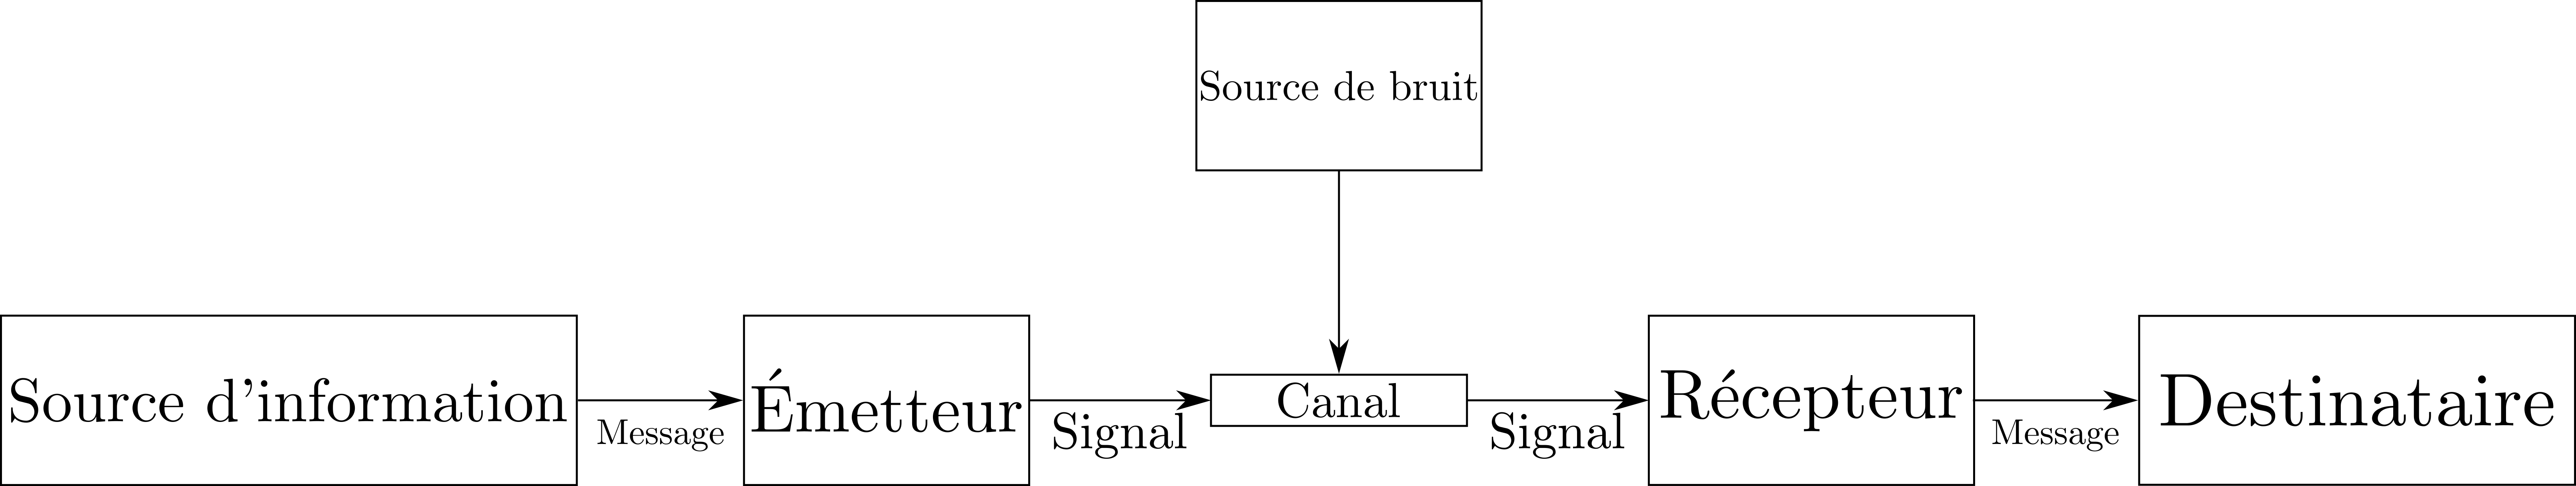
\includegraphics[scale=0.3]{images/schema_contexte_detection_general.png}
            \end{center}
        }

        \only<2>{
            \begin{center}
                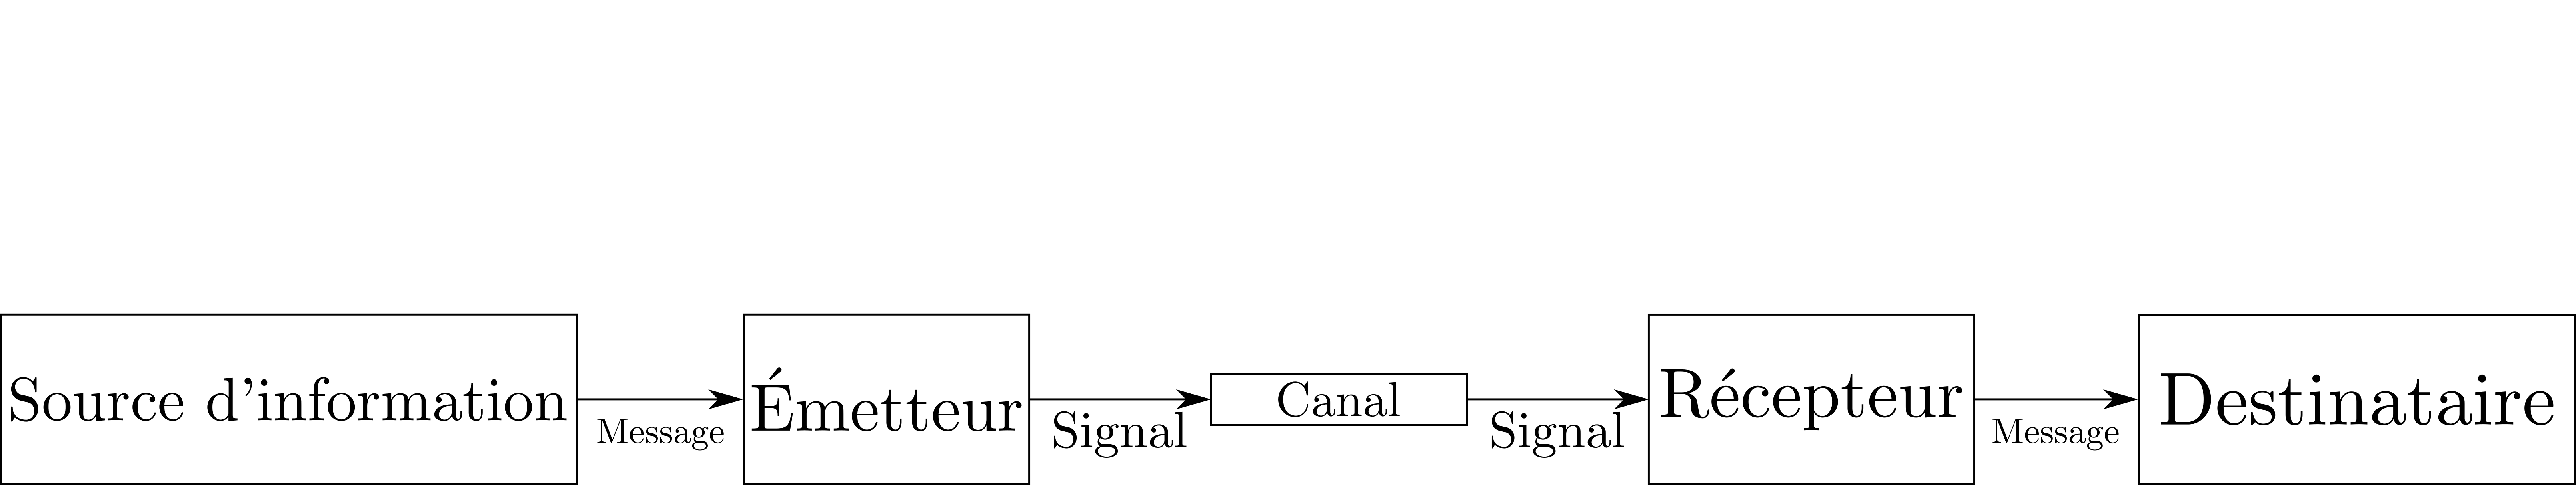
\includegraphics[scale=0.3]{images/schema_contexte_detection_general_2.png}
            \end{center}
        }

        \only<3>{
            \begin{center}
                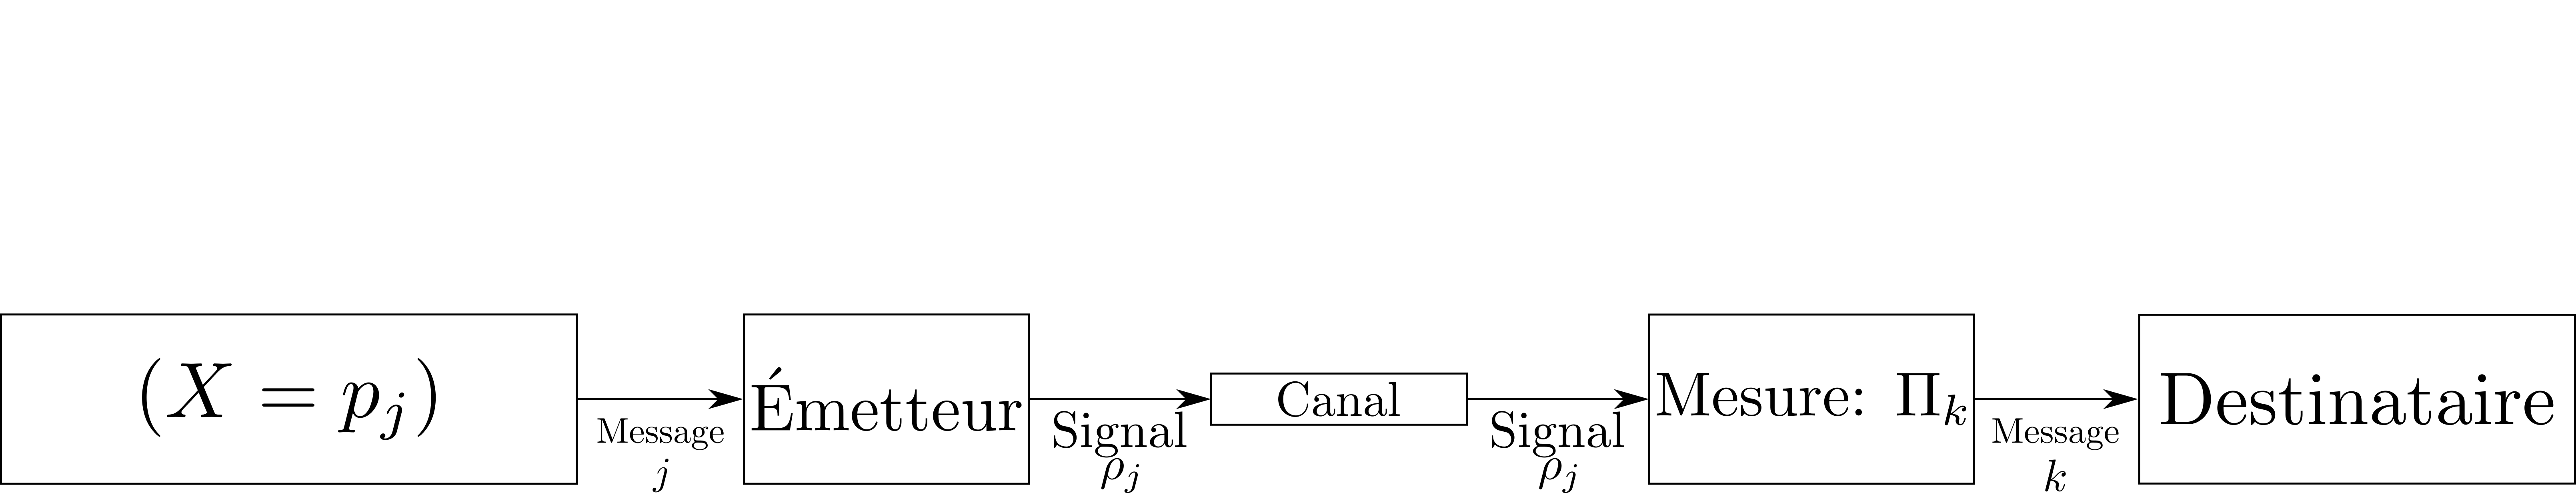
\includegraphics[scale=0.3]{images/schema_contexte_detection_general_3.png}
            \end{center}
        }

        \small
        \only<1,2>{
            Problème classique du traitement de l'information: détection optimale.
        }
        \only<3>{
            Cas quantique: ensemble d'états quantiques $\rho_j$, ayant une probabilité $p_j$, mesurés avec un opérateur de mesure $\Pi_k$.
        }
    \end{block}

    % \begin{block}{}
    %     \begin{center}
    %         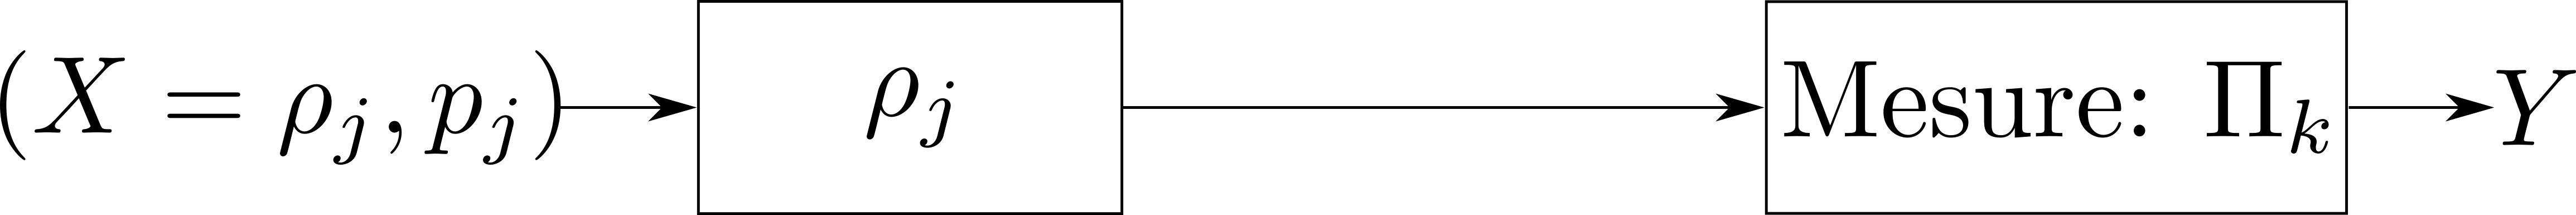
\includegraphics[scale=0.3]{images/schema_contexte_detection.png}
    %     \end{center}
    %     \small
        
    % \end{block}

    % \tableofcontents
    % \begin{block}{}
    %     On se place dans le problème de base du traitement du signal quantique consistant en la conception d'un détecteur quantique optimal maximisant la performance de détection d'un état parmi une famille d'états quantique, chaucn étant représenté par un opérateur densité $\rho_j$ et ayant une probabilité à priori $p_j$, étant mesuré via un opérateur de mesure $\Pi_k$.

    %     % \'Etant donné cette famille d'opérateurs densité $\{\rho_j, 1 \leq j \leq m\}$ et leur probabilités à priori, la famille d'opérateurs de mesure $\{\Pi_k, 1 \leq k \leq n \}$ permet de délivrer une certaine mesure $k$.
    % \end{block}
\end{frame}

\begin{frame}
    \tableofcontents
\end{frame}

\section[1. Système quantique]{Système quantique}
\subsection{\'Etat d'un système quantique}

\begin{frame}
    \frametitle{1.1: \'Etat d'un système quantique}
    \only<1>{
    \begin{block}{Définition: état d'un système quantique} % Changer de "definition" à "définition"
      Système quantique \textbf{pur}: vecteur d'état $\ket{\psi}$ 
      
      \begin{itemize}
        \item dans un espace de Hilbert complexe $\mathcal{H}$,
        \item de norme unité: $||\psi||^2 = \braket{\psi | \psi} = 1$,
        \item avec des coordonnées: \begin{equation} \ket{\psi} = \displaystyle\sum_{i} c_i \ket{k_i}, \end{equation}
        \item où $\{\ket{k_i}\}_i$ une base orthonormée de $\mathcal{H}$,
        \item et les coefficients $c_i \in \mathbb{C}$.
      \end{itemize}
    
    \end{block}
    }
\end{frame}

\begin{frame}
    \frametitle{1.1: \'Etat d'un système quantique}
    \small

    \begin{block}{Définition: opérateur densité}
        \textit{Opérateur densité} : matrice Hermitienne $\rho$, telle que $\rho = \rho^{\dagger}$, $\tr(\rho) = 1$ et $\rho \succeq 0$.
    \end{block}

    \pause

    \begin{block}{}

        \'Etat \textbf{pur}: opérateur densité $\rho_j = \ket{\psi_j} \bra{\psi_j}.$
        \medbreak

        \'Etat \textbf{mélangé}: opérateur densité $\rho_j$ non représentable en vecteur d'état.
    \end{block}

    \pause

    \begin{block}{Exemple}
        Soit un état quantique $\ket{\psi_j} = \ket{+} = 
        \begin{pmatrix}
            \frac{1}{\sqrt{2}} \\ \frac{1}{\sqrt{2}}
        \end{pmatrix}.$

        L'opérateur densité correspondant est : $\rho_j = \ket{\psi_j}\bra{\psi_j} =\begin{pmatrix} \frac{1}{\sqrt{2}} \\ \frac{1}{\sqrt{2}} \end{pmatrix} \begin{pmatrix} \frac{1}{\sqrt{2}} & \frac{1}{\sqrt{2}} \end{pmatrix} = \begin{pmatrix} 0.5 & 0.5 \\ 0.5 & 0.5 \end{pmatrix}. \nonumber
        $
    \end{block}
\end{frame}

\subsection{Mesure quantique}

\begin{frame}
    \frametitle{1.2: Mesure quantique}
    % \footnote{Chapeau-Blondeau, F., "Quantum information, quantum computation : An introduction", Cours de formation doctorale (2018)}

    \begin{block}{Définition: Mesure projective}
        Mesure projective: $N$ projecteurs orthogonaux $\ket{n}\bra{n} = \Pi_n$, tels que $\displaystyle \sum_n\ket{n}\bra{n} = \displaystyle \sum_n \Pi_n = I_N$ et $Pr\{\ket{n}\} = \tr(\rho \Pi_n)$.
    \end{block}

    \pause

    \begin{block}{Définition: Mesure généralisée (POVM)}
        POVM: \textit{Positive Operator-Valued Measurement}, $K$ opérateurs de mesure non nécessairement projecteurs orthogonaux $\{\Pi_k\}$, tels que $\sum_k \Pi_k = I_k$ et $Pr\{\Pi_k\} = \tr(\rho \Pi_k)$.
    \end{block}
\end{frame}

\subsection{Problème de la mesure optimale}

\begin{frame}
    \frametitle{1.3: Problème de la mesure optimale}

    \begin{block}{Problème à résoudre}
        Obtenir les $\{\Pi_k\}$ opérateurs de mesure permettant d'identifier le mieux possible les états d'entrée $\{\rho_j\}$.
    \end{block}

    \pause

    \begin{block}{Critères d'optimisation}
        \begin{enumerate}
            \item Maximiser la probabilité de détection correcte (linéaire), \footnote{\tiny Eldar, Y., "Designing Optimal Quantum Detectors Via Semidefinite Programming", IEEE Transaction on Information Theory 49 (2003), 1012-1017}
            \item Minimiser l'erreur quadratique de mesure, \footnote{\tiny Eldar, Y., "On Quantum Detection and the Square-Root Measurement", IEEE Transaction on Information Theory 47 (2001), 858-872}
            \item Maximiser information mutuelle (non linéaire) \footnote{\tiny Davies, E., "Information and quantum measurement", IEEE Transaction on Information Theory 24 (1978), 596-599}.
        \end{enumerate}
    \end{block}
\end{frame}

\begin{frame}
    \frametitle{1.3: Problème de la mesure optimale}

    \only<1>{
        \small
        \begin{block}{Définition: information mutuelle}

            L'\textit{information mutuelle} est définie pour deux variables aléatoires $X$ et $Y$ par:

            \begin{align}
                I(X; Y) &= H(X) + H(Y) - H(X, Y) \\
                &= H(Y) - H(Y | X) \\
                &= H(X) - H(X | Y)
            \end{align}

            \begin{columns}
                \begin{column}{0.5\textwidth}
                    \tiny
                    \begin{enumerate}
                        \item $H(X)$ et $H(Y)$ entropies marginales de $X$ et $Y$; 
                        \item $H(X, Y)$ entropie conjointe de $X$ et $Y$;
                        \item $H(X|Y)$ entropie de $X$ sachant $Y$.
                    \end{enumerate}
                \end{column}
                \begin{column}{0.5\textwidth}
                    \tiny
                    \begin{align*}
                        X &= \{ \rho_j = \ket{\phi_j}\bra{\phi_j}, 1 \leq j \leq m\}, \nonumber\\
                        Y &= \{ \Pi_k  = \ket{\mu_k}\bra{\mu_k}, 1 \leq k \leq m\} \nonumber
                    \end{align*}
                    Avec $\{p_j\}$ distribution marginale de $X$.
                \end{column}
            \end{columns}

        \end{block}
    }

    \only<2>{
        \begin{columns}
            \small
            \begin{column}{0.5\textwidth}
                \begin{block}{Problème}
                    On cherche à résoudre le problème de maximisation :
                    \begin{align}
                        \max\limits_{\{\Pi\}} I(\rho, \Pi)
                    \end{align}
        
                    tel que :
        
                    \begin{align}
                        \Pi_j \succeq 0, \quad 1 \leq j \leq m \label{eq:contrainte_sdp} \\
                        \displaystyle \sum_{j=1}^{m} \Pi_j = I \label{eq:contrainte_somme_id}
                    \end{align}
                \end{block}
            \end{column}
            \begin{column}{0.5\textwidth}
                \begin{figure}[H]
                    \centering
                    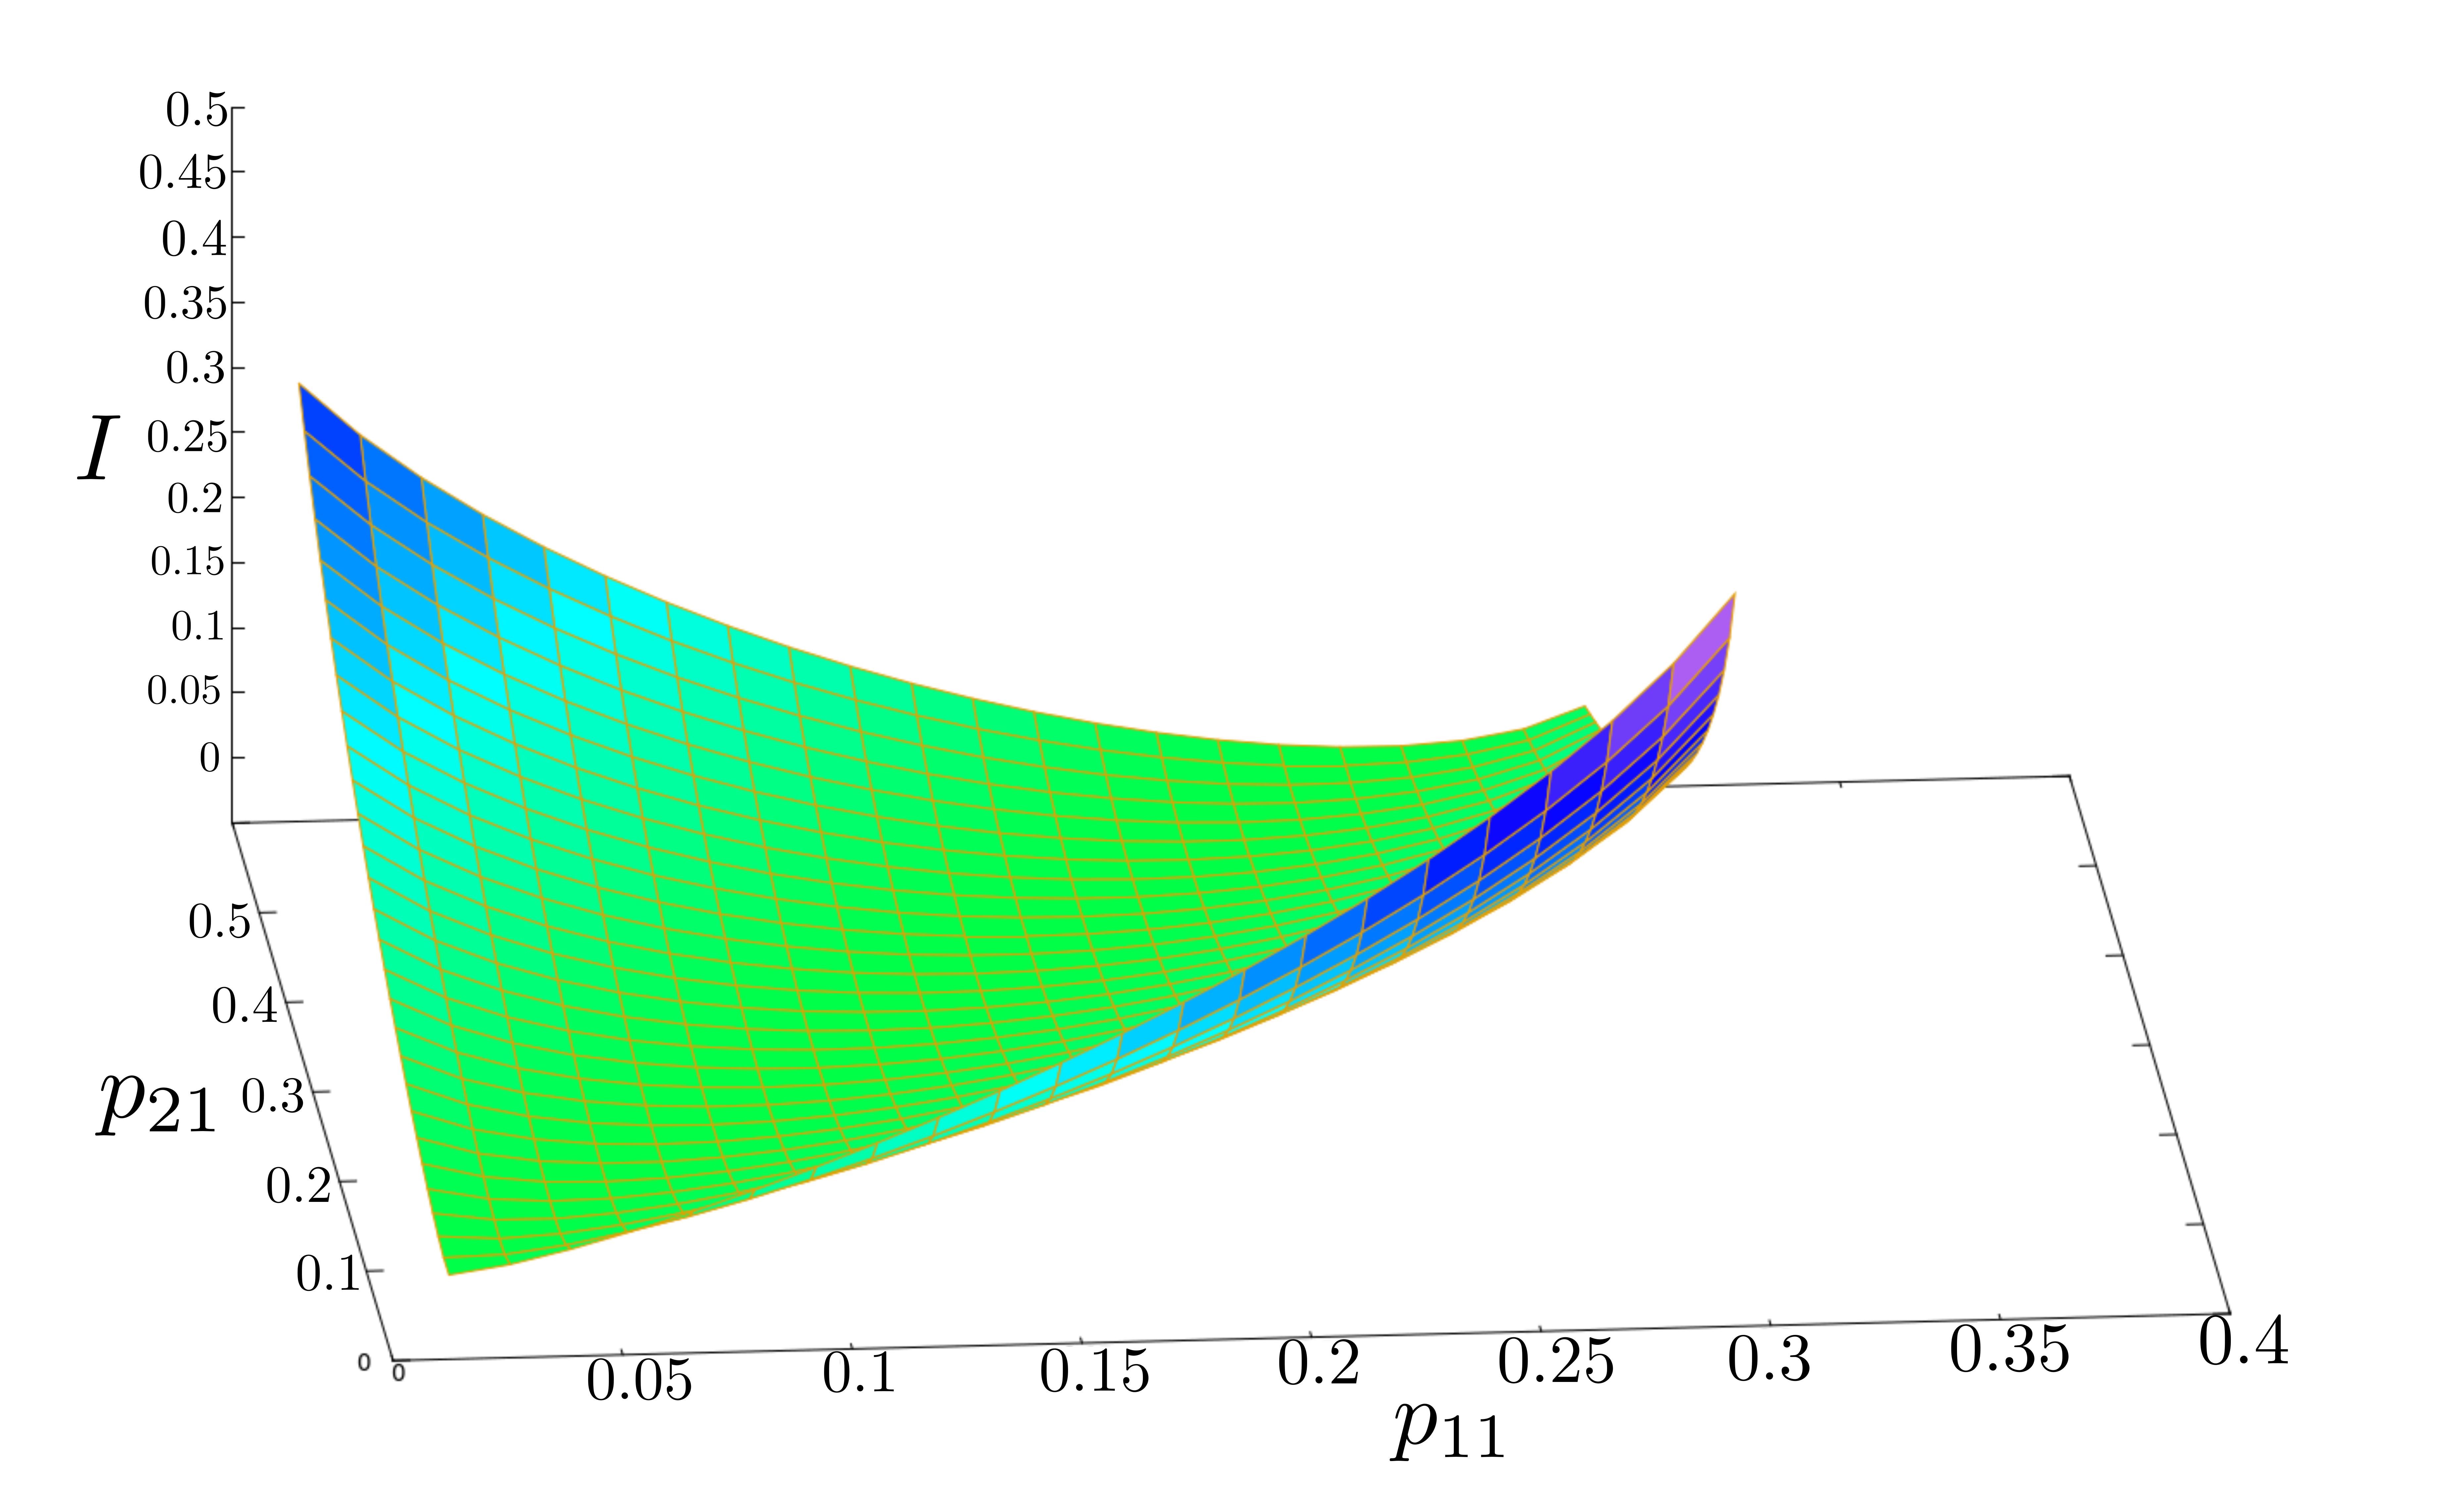
\includegraphics[scale=0.13]{images/MI_convex.png}
                    \caption{}
                    \label{fig:mi_convex}
                \end{figure}
            \end{column}
        \end{columns}


        \begin{itemize}
            \item Problème de maximisation de fonction non linéaire, convexe: difficile en pratique à résoudre.
            \item Utilisation du calcul par intervalle pour fournir une solution optimale garantie.
        \end{itemize}
    }
\end{frame}

\section[2. Calcul par intervalles]{Optimisation via le calcul par intervalle}
\subsection{Intervalle et fonction d'inclusion}
\begin{frame}
    \frametitle{2.1: Intervalle et fonction d'inclusion}
    \begin{block}{Notion d'intervalle}
        Un intervalle $\textbf{x} = [\underline{x}, \overline{x}]$ est défini comme l'ensemble des nombres réels $x$ t.q. $\underline{x} \leq x \leq \overline{x}$. 
    \end{block}

    % \pause

    % \begin{block}{Notion de boites}
    %     Une boite $\textbf{X} = (\textbf{x1}, \textbf{x2}, ..., \textbf{xj})$ est le produit cartésien des intervalles $\textbf{x1} \times \textbf{x2} \times \dots \times \textbf{xj}$
    % \end{block}
    % \pause

    % \begin{figure}[H]
    %     \centering
    %     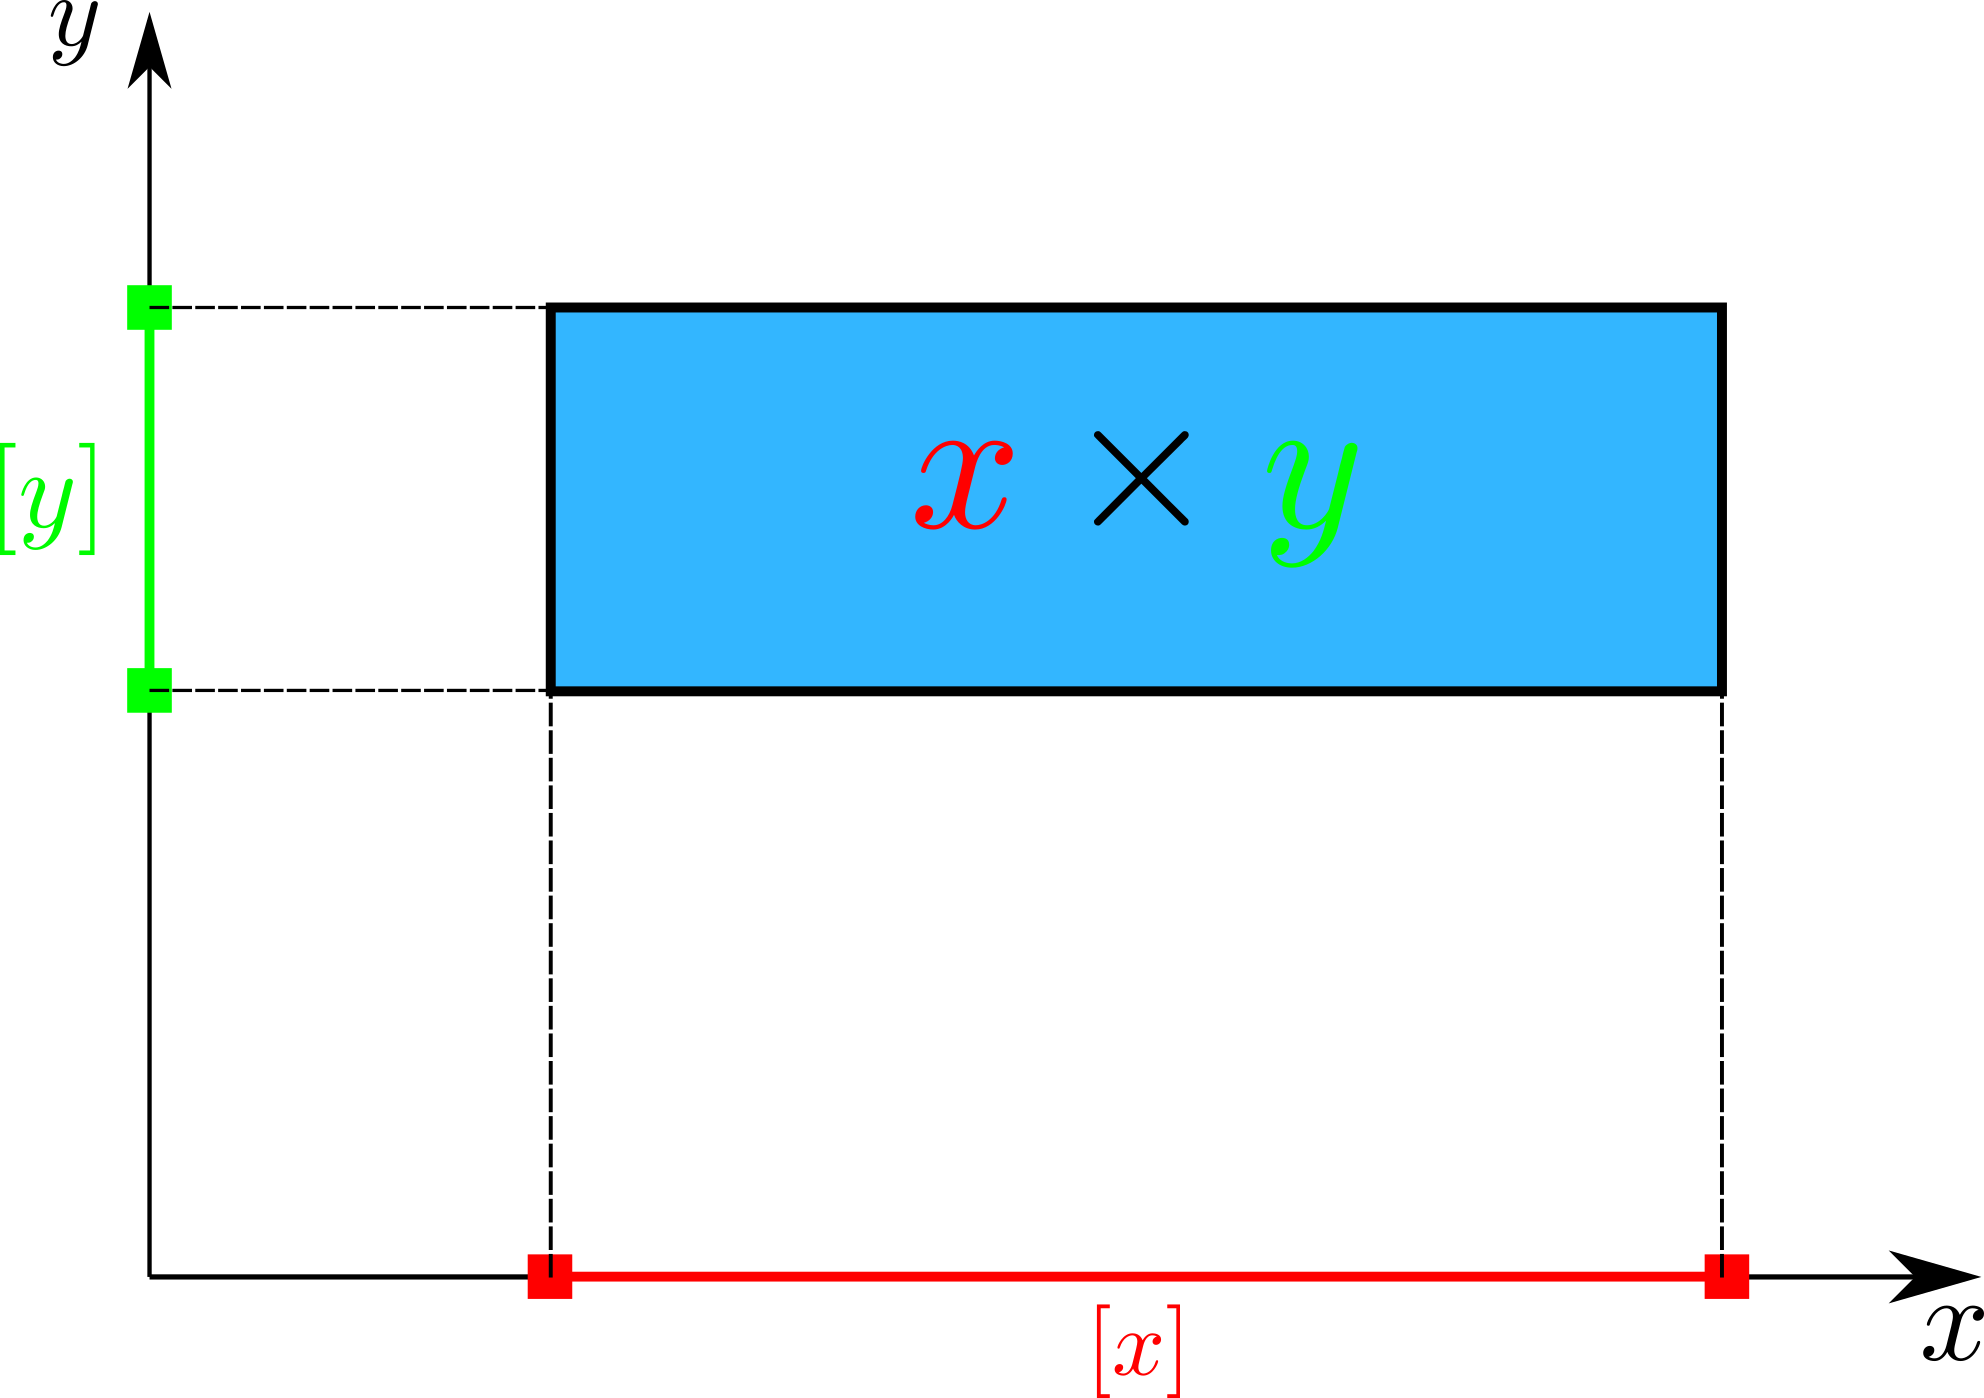
\includegraphics[scale=0.5]{images/box.png}
    %     \caption{}
    %     \label{fig:box}
    % \end{figure}
\end{frame}

\begin{frame}
    \frametitle{2.1: Intervalle et fonction d'inclusion}

    \begin{block}{Définition: fonction d'inclusion}
        Soit $f : \mathbb{R}^n \rightarrow \mathbb{R}^m$ une fonction, la fonction $[f] : \mathbb{R}^n \rightarrow \mathbb{R}^m$ est une \textit{fonction d'inclusion} pour $f$ si

        \begin{align}
            \forall[\underline{x}, \overline{x}] \in \mathbb{R}^n , f([\underline{x}, \overline{x}]) \subset [f]([\underline{x}, \overline{x}])
        \end{align}
    \end{block}

    \only<1>{
        \begin{figure}[H]
            \centering
            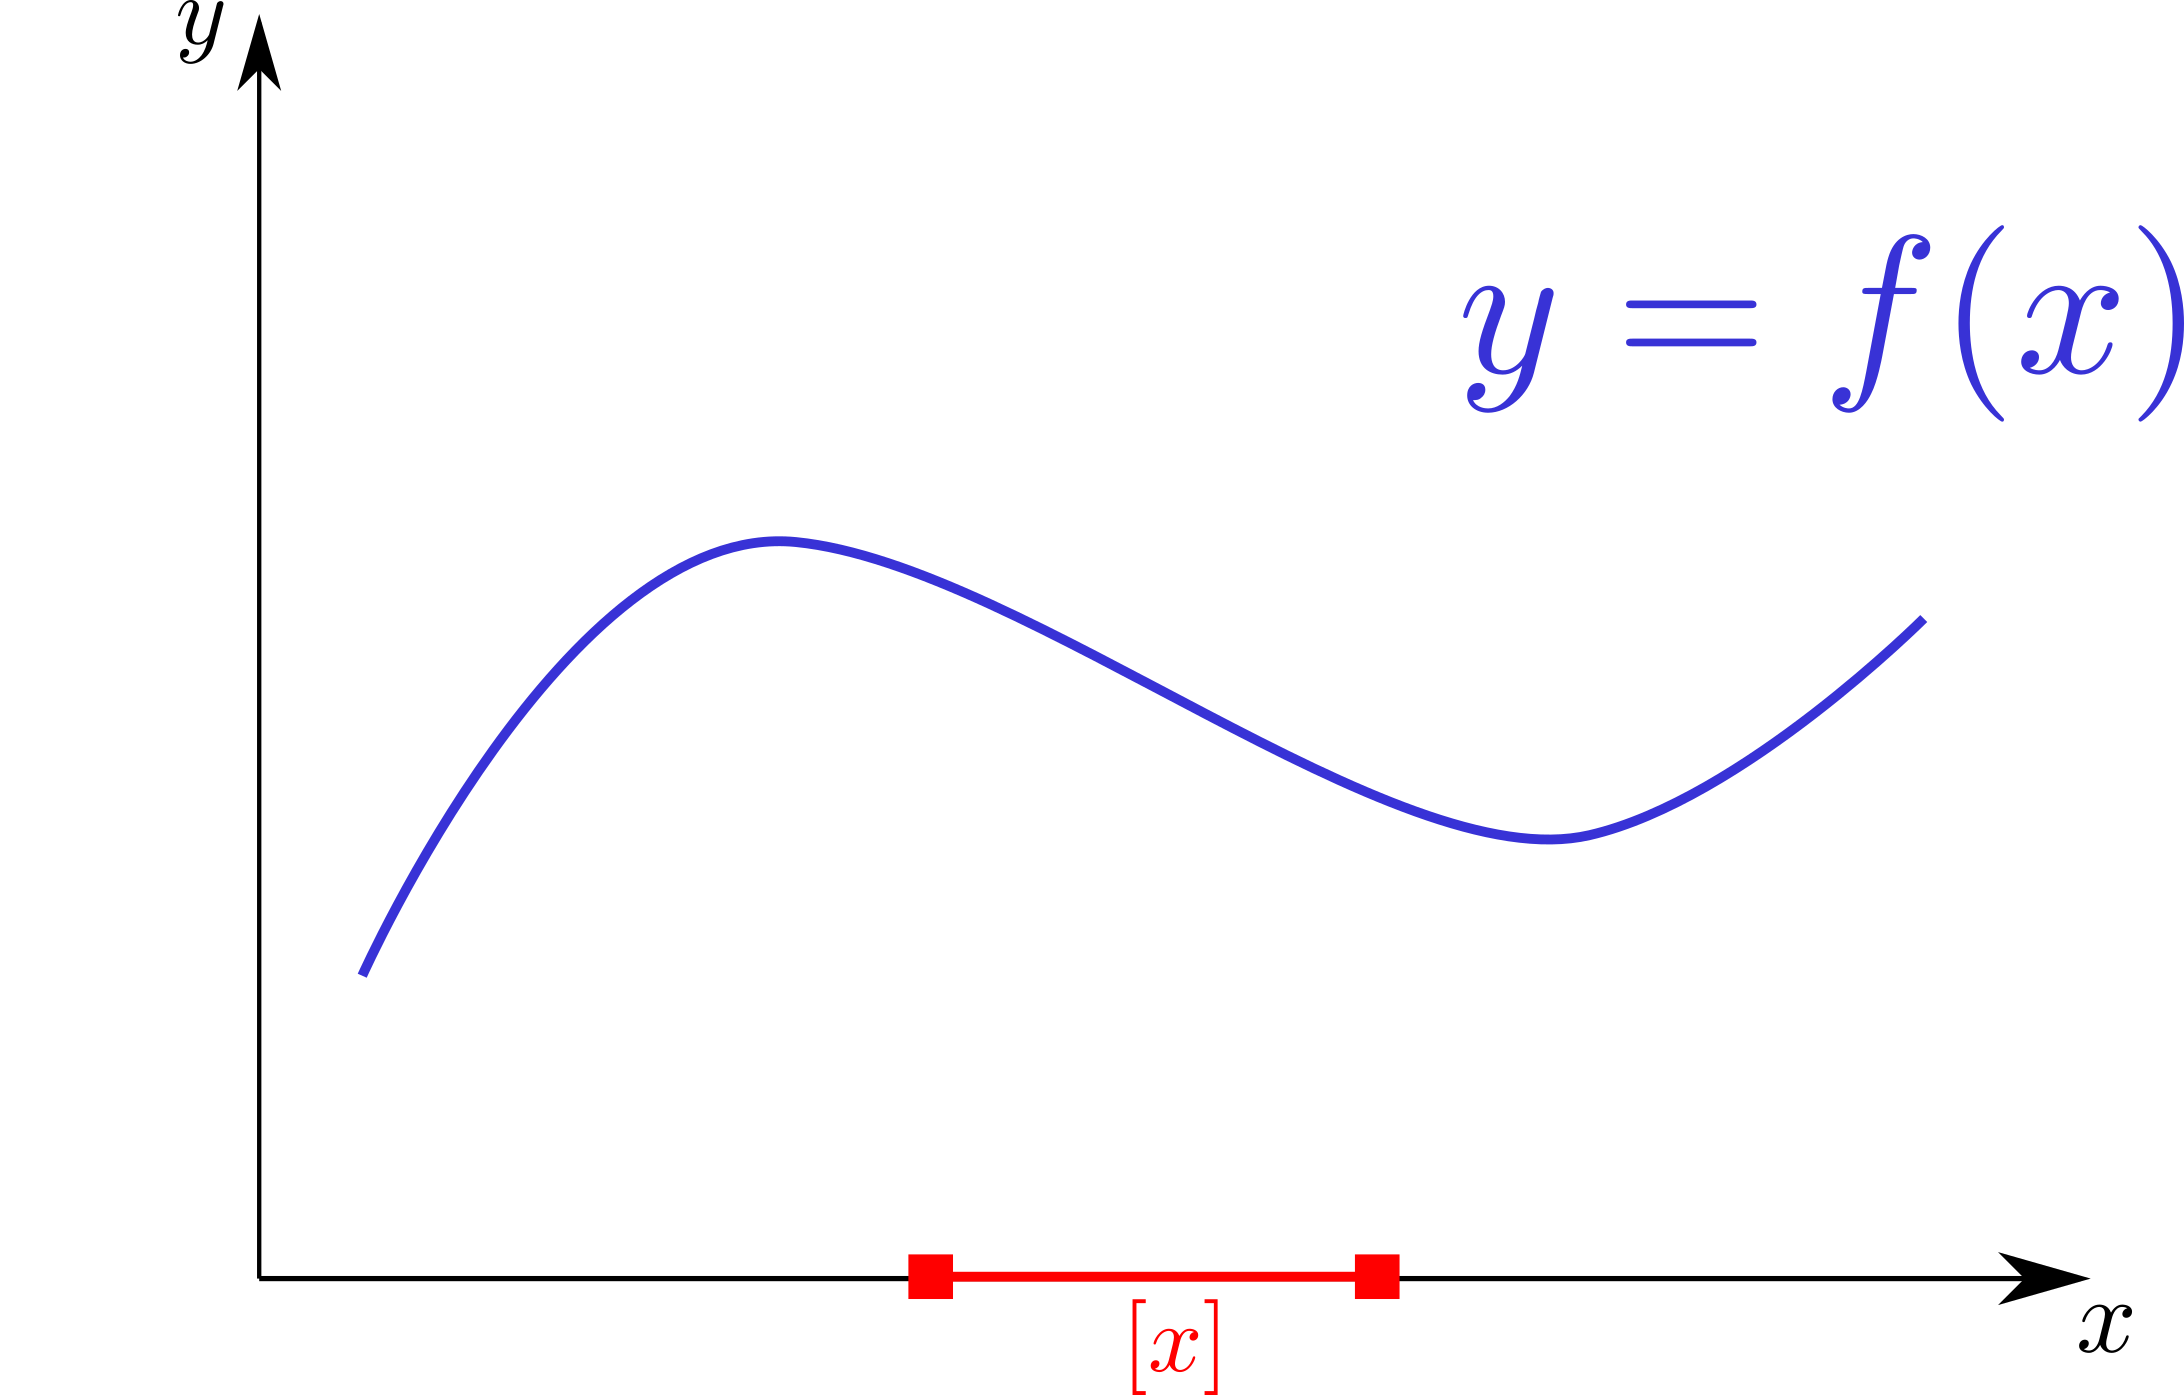
\includegraphics[scale=0.5]{images/function_eval_1.png}
            \caption{}
            \label{fig:fct1}
        \end{figure}
    }
    \only<2>{
        \begin{figure}[H]
            \centering
            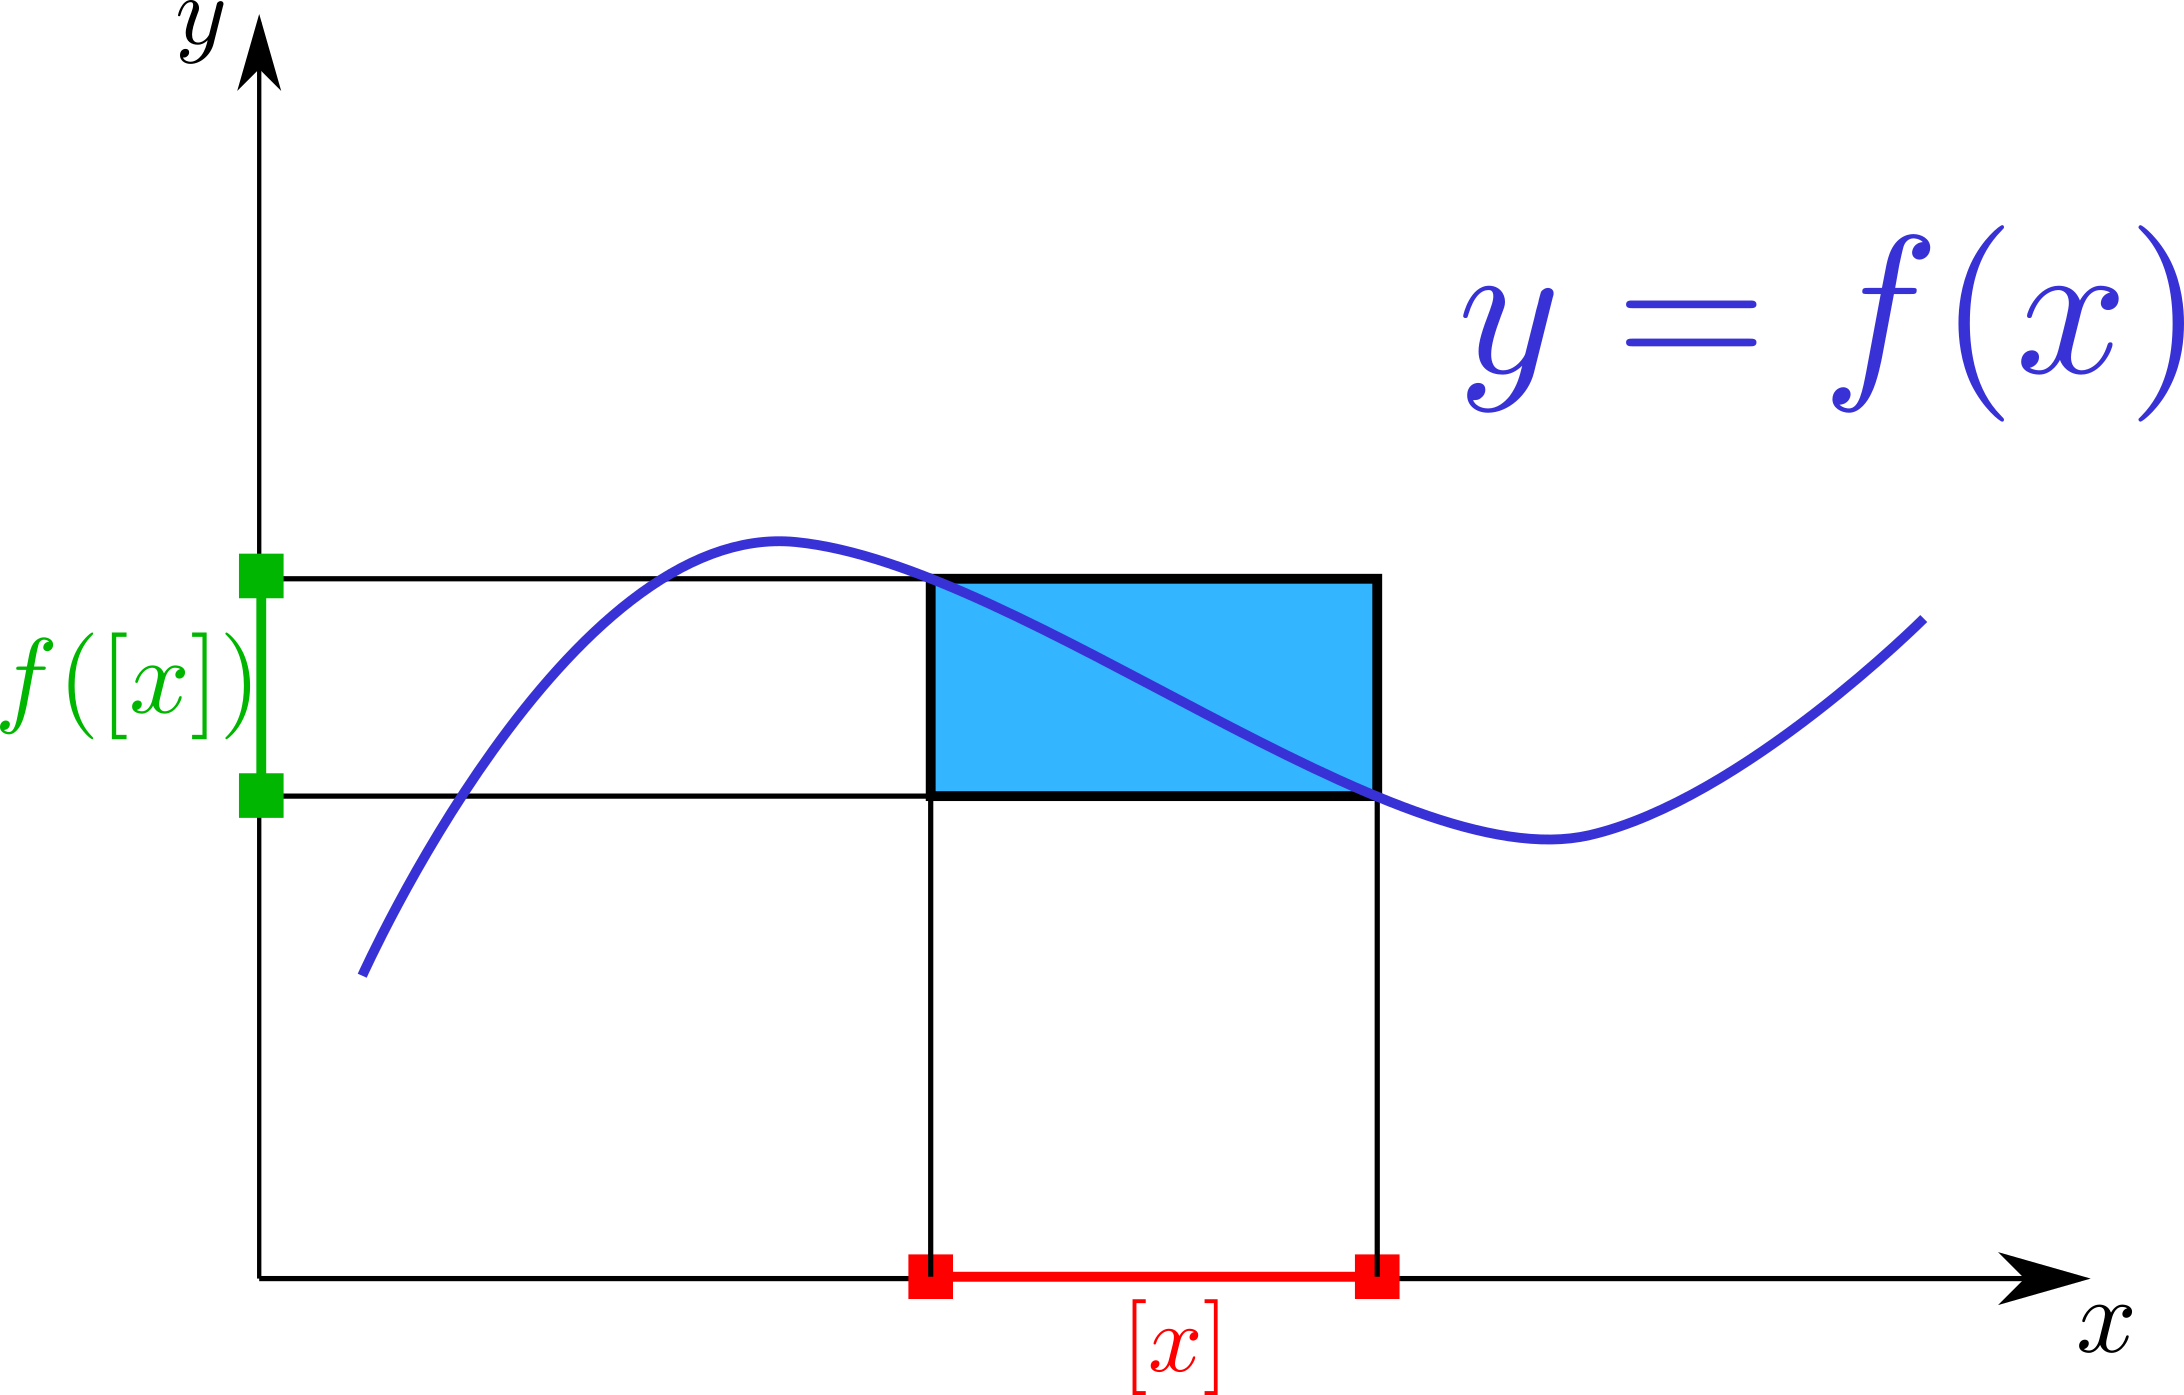
\includegraphics[scale=0.5]{images/function_eval_2.png}
            \caption{}
            \label{fig:fct2}
        \end{figure}
    }
    \only<3>{
        \begin{figure}[H]
            \centering
            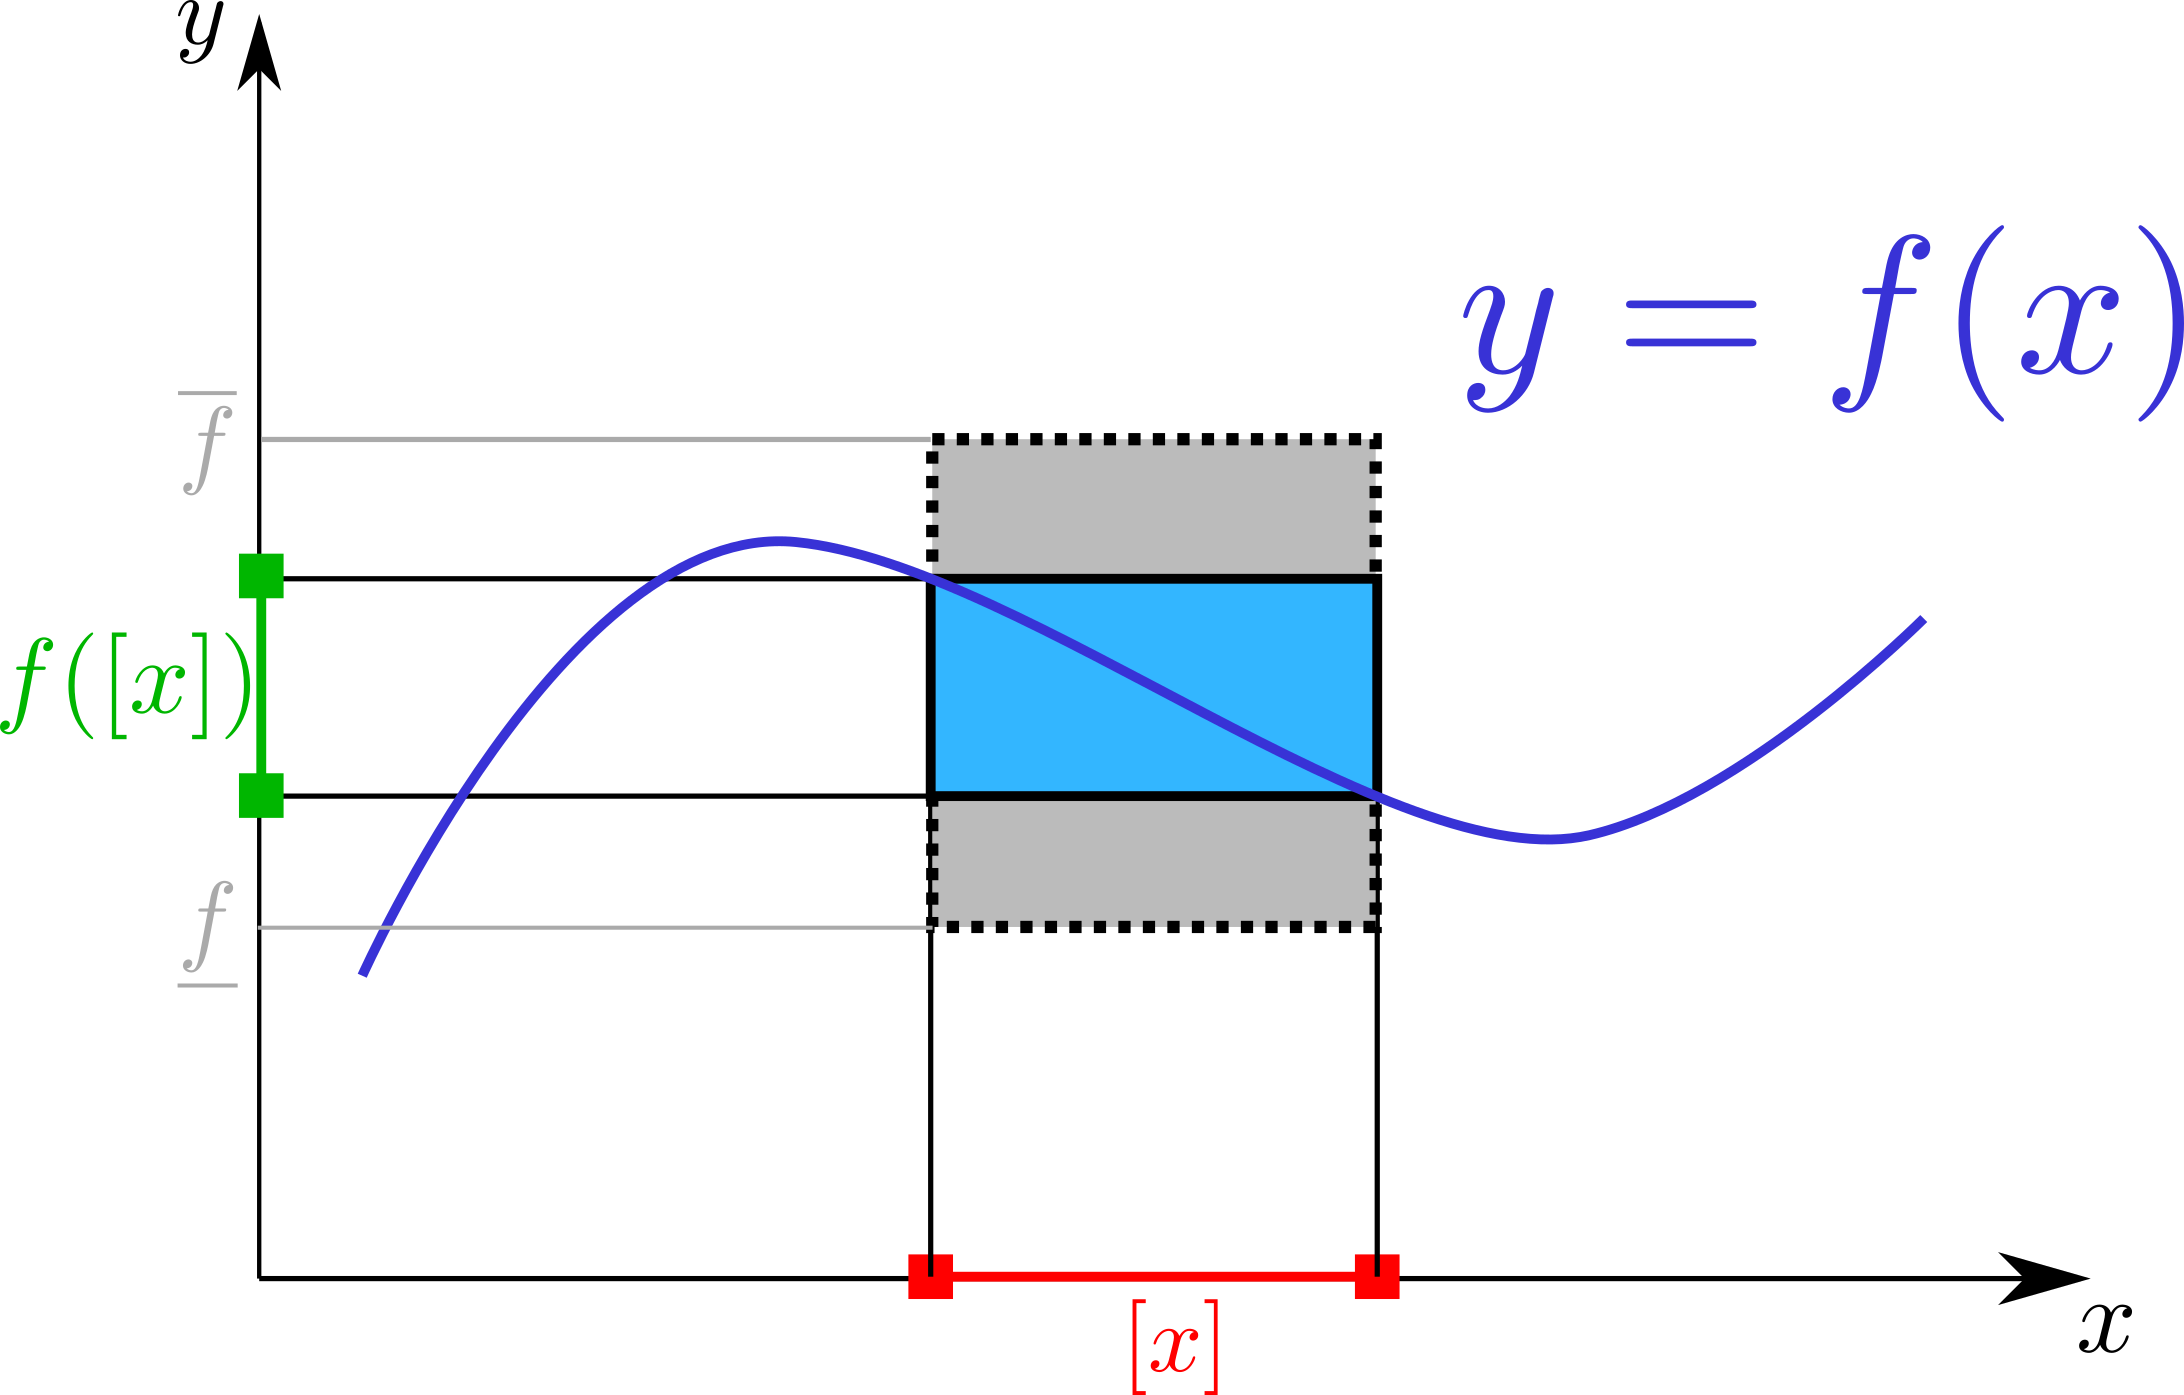
\includegraphics[scale=0.5]{images/function_eval_3.png}
            \caption{}
            \label{fig:fct3}
        \end{figure}
    }
\end{frame}


\begin{frame}
    \frametitle{2.1: Intervalle et fonction d'inclusion}
    On définit un ensemble d'opérateurs comme extension des opérateurs arithmétiques sur les nombres réels:

    \small
    \begin{itemize}
        \item $[x_1] + [x_2] = [\underline{x_1} + \underline{x_2}, \overline{x_1} + \overline{x_2}]$
        \item $[x_1] - [x_2] = [\underline{x_1} - \overline{x_2}, \overline{x_1} - \underline{x_2}]$
        \item $[x_1] \times [x_2] = [\text{min}(\underline{x_1}\underline{x_2}, \underline{x_1}\overline{x_2}, \overline{x_1}\underline{x_2}, \overline{x_1}\overline{x_2}), \text{max}(\underline{x_1}\underline{x_2}, \underline{x_1}\overline{x_2}, \overline{x_1}\underline{x_2}, \overline{x_1}\overline{x_2})]$
        \item $\log([x]) = [\log(\underline{x_1}), \log(\overline{x_2})]$
        \item \dots
    \end{itemize}

    \begin{block}{Exemple}
        \begin{align}
            [z] &= ([2, 3] - [-4, 5])^2 + [-3, 2] \nonumber \\
                &= [-3,7]^2 + [-3, 2] \nonumber \\
                &= [0, 49] + [-3, 2] \nonumber \\
                &= [-3, 51] \nonumber
        \end{align}
    \end{block}
\end{frame}

\subsection{Algorithmes d'optimisation par intervalles}

\begin{frame}
    \frametitle{2.2: Algorithmes d'optimisation par intervalles}
    \begin{block}{Théorème}
        Soit un $a$ une solution admissible du problème $\max\limits_{x} f(x)$ tel que $g(x) \leq 0$ et $x^*$ la solution optimale, on a:
        \begin{align}
            sup([f]([x])) \leq f(a) \Rightarrow x^* \notin [x]
        \end{align}
    \end{block}

    \only<1>{
        \begin{figure}[H]
            \centering
            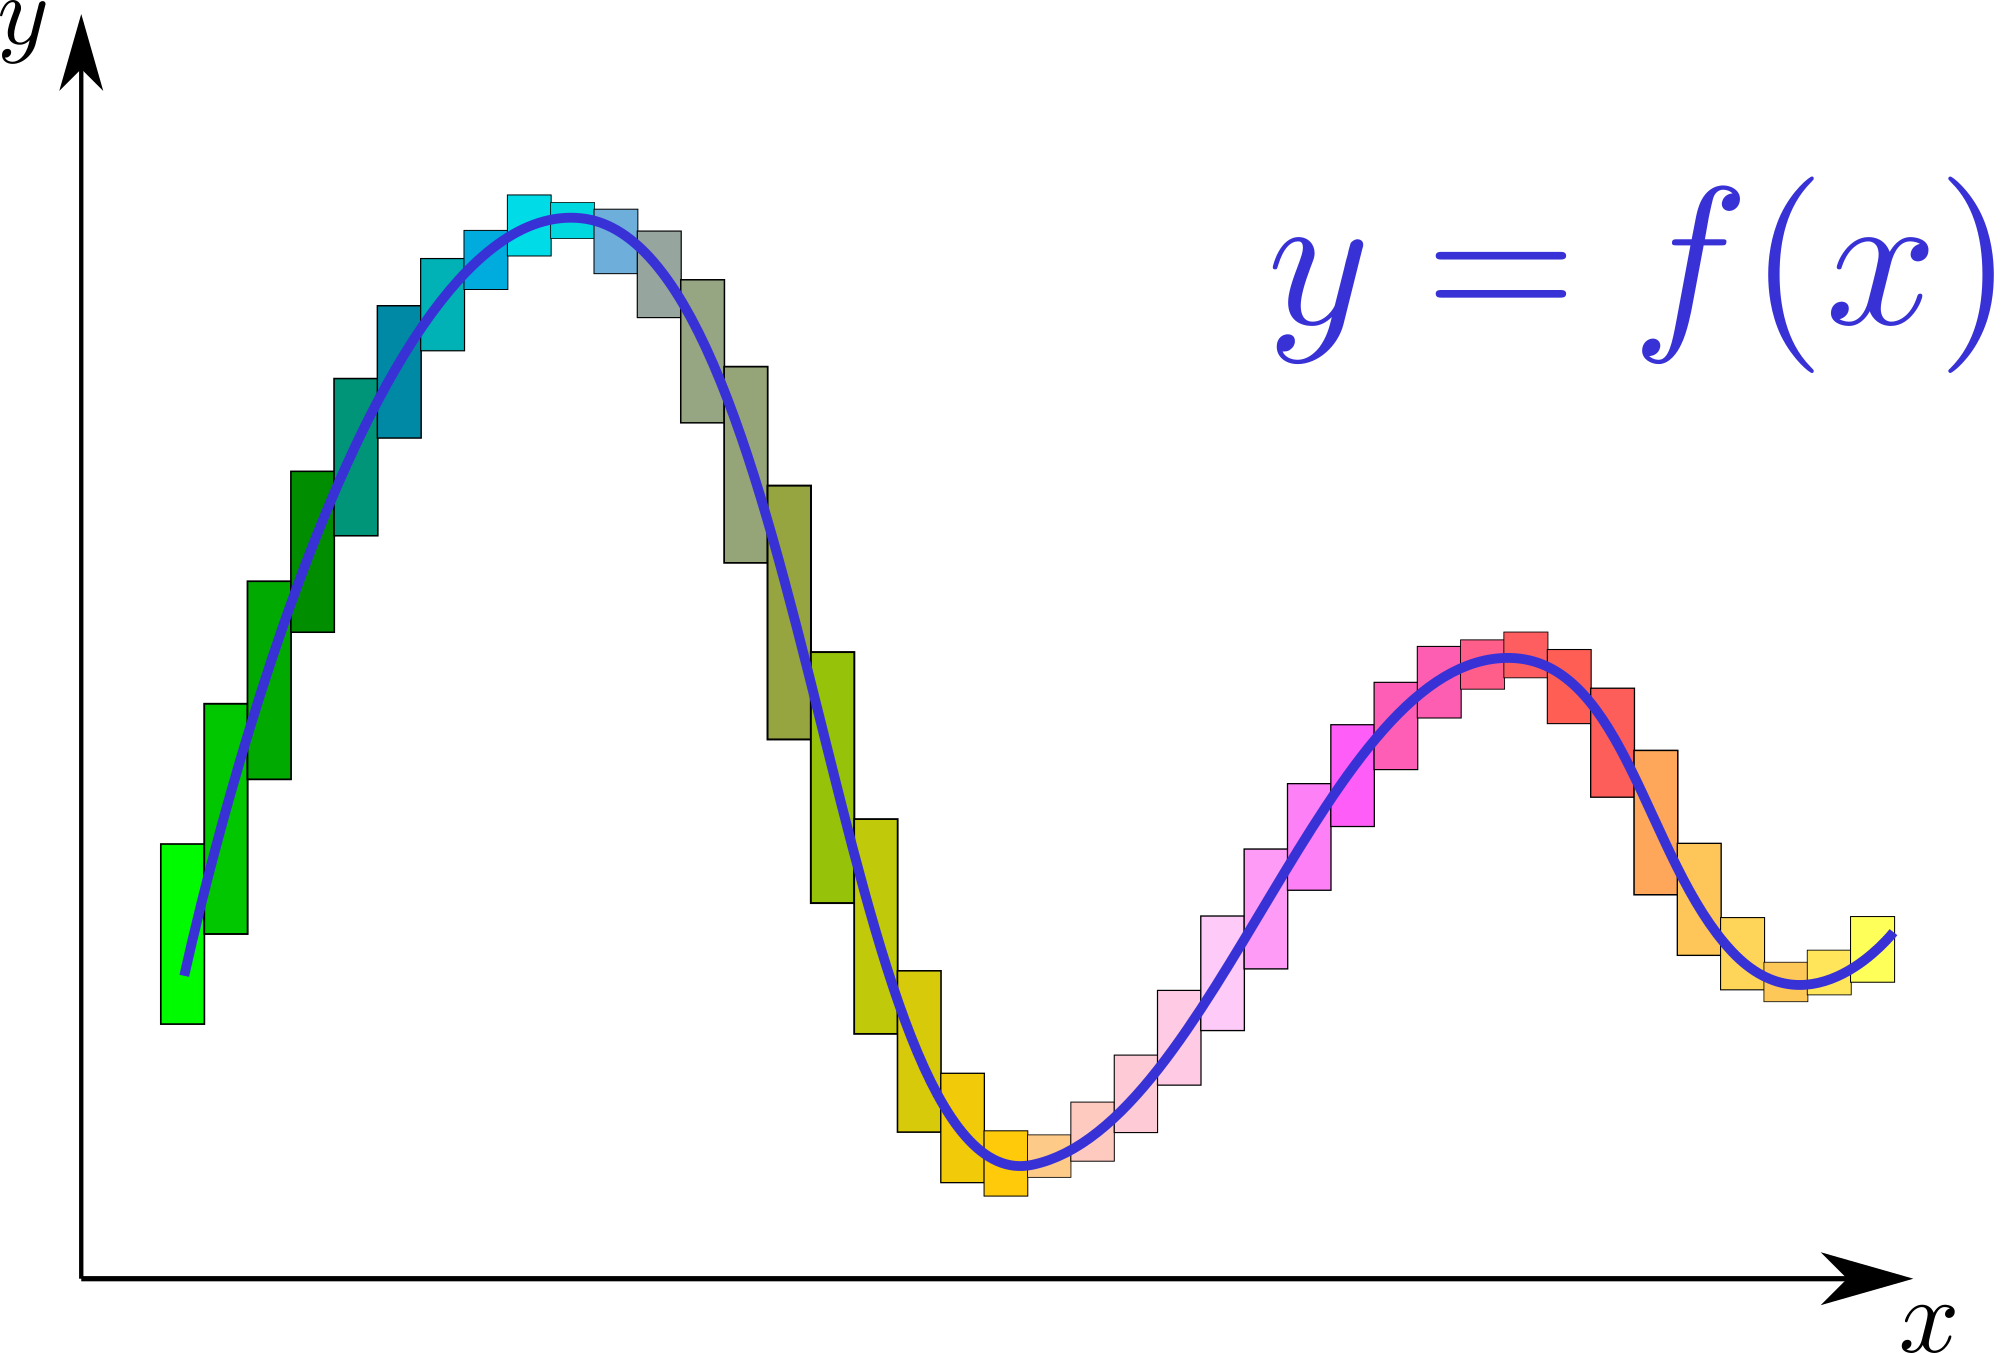
\includegraphics[scale=0.5]{images/function_optim_1.png}
            \caption{$y = f(x)$}
            \label{fig:optim1}
        \end{figure}
    }

    \only<2>{
        \begin{figure}[H]
            \centering
            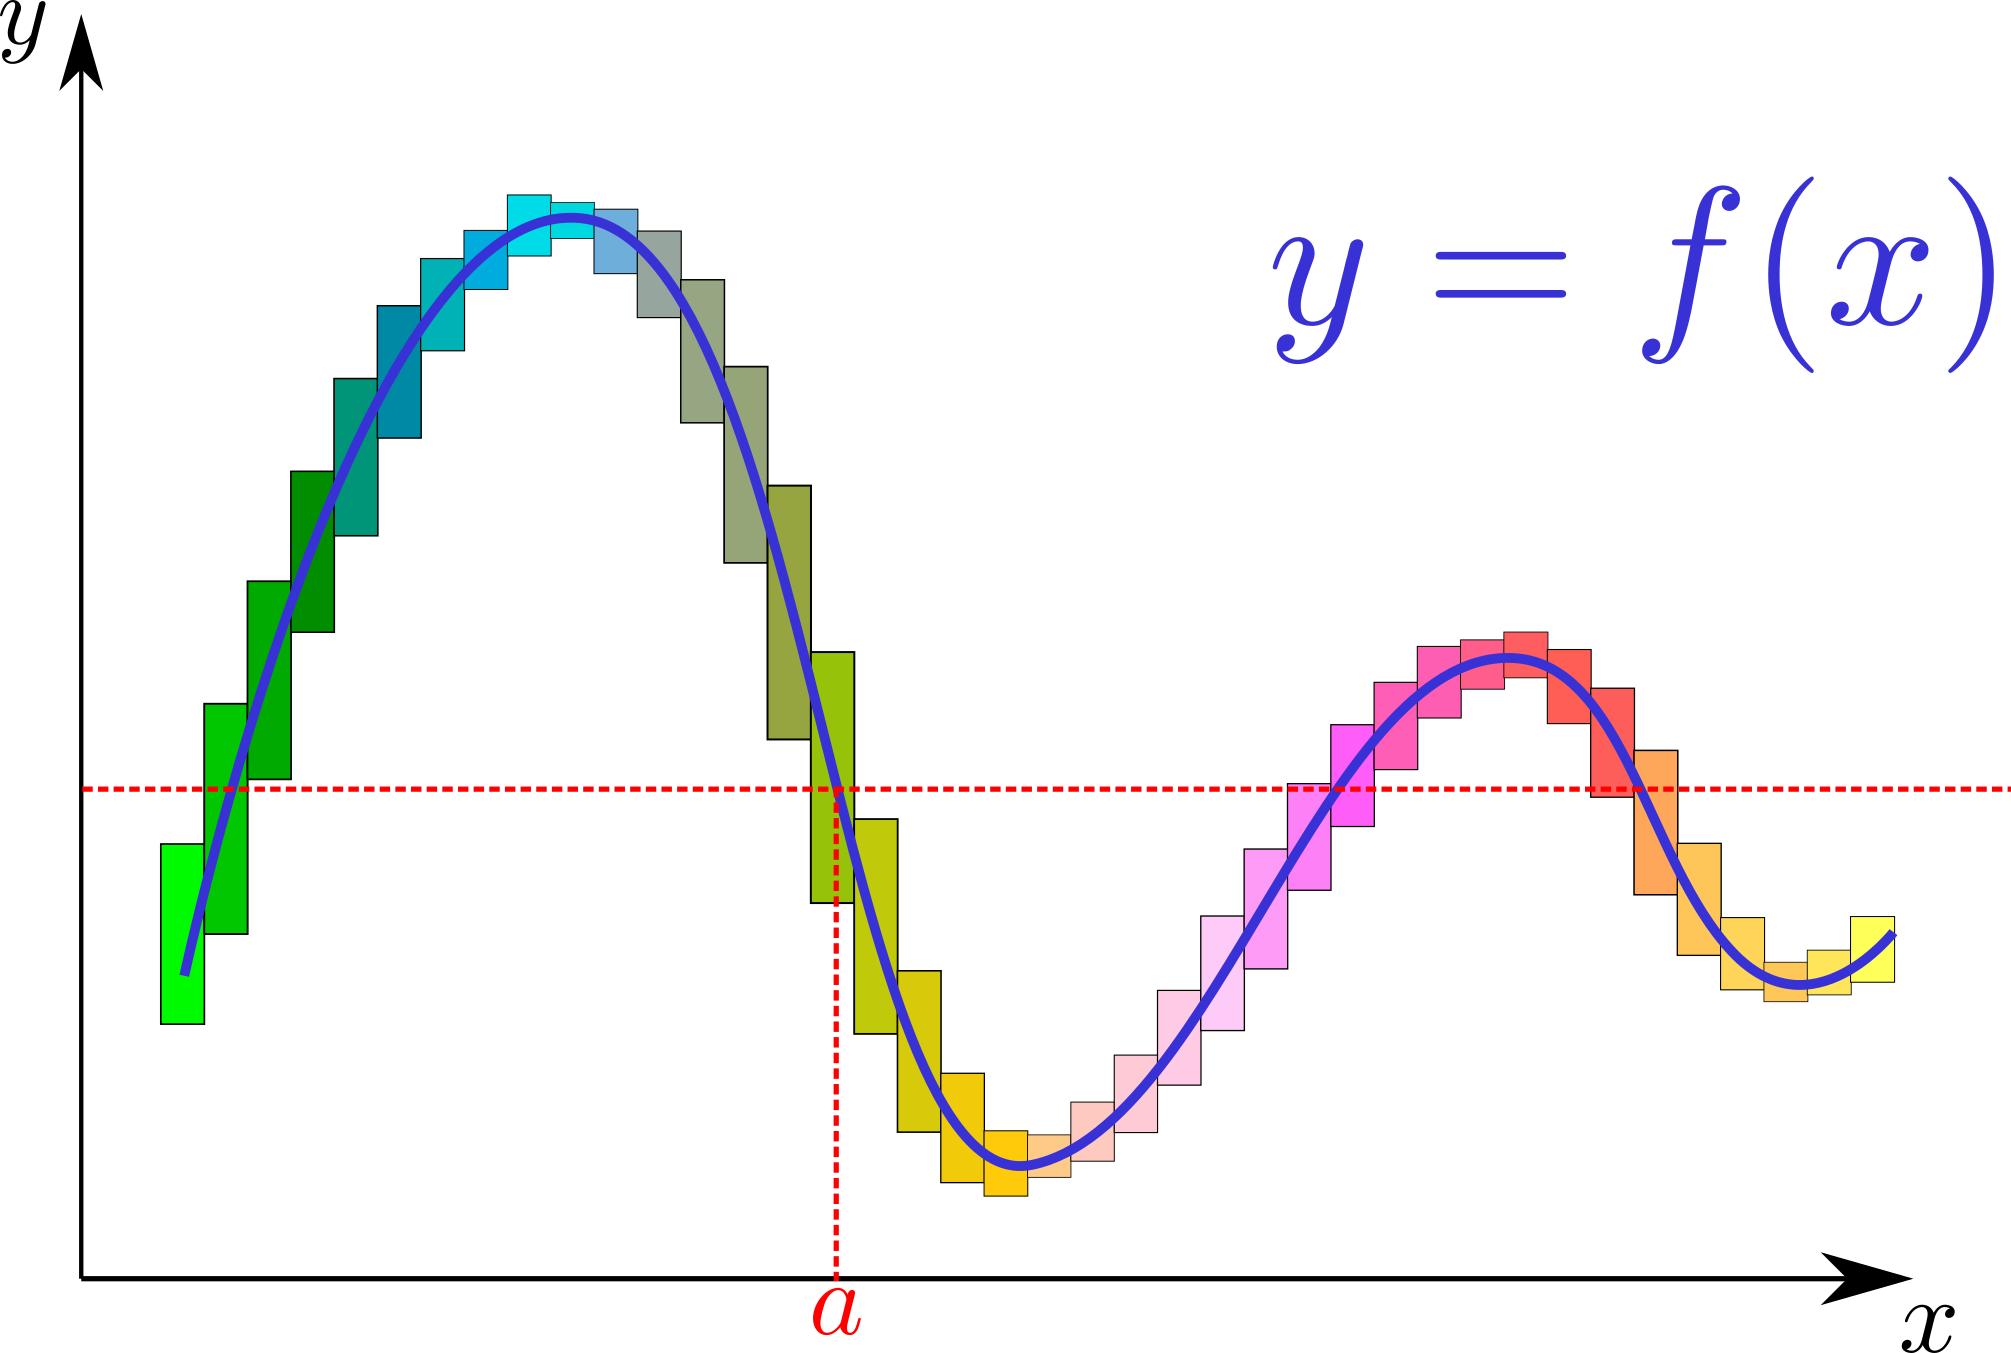
\includegraphics[scale=0.5]{images/function_optim_2.png}
            \caption{$y = f(x)$}
            \label{fig:optim2}
        \end{figure}
    }

    \only<3>{
        \begin{figure}[H]
            \centering
            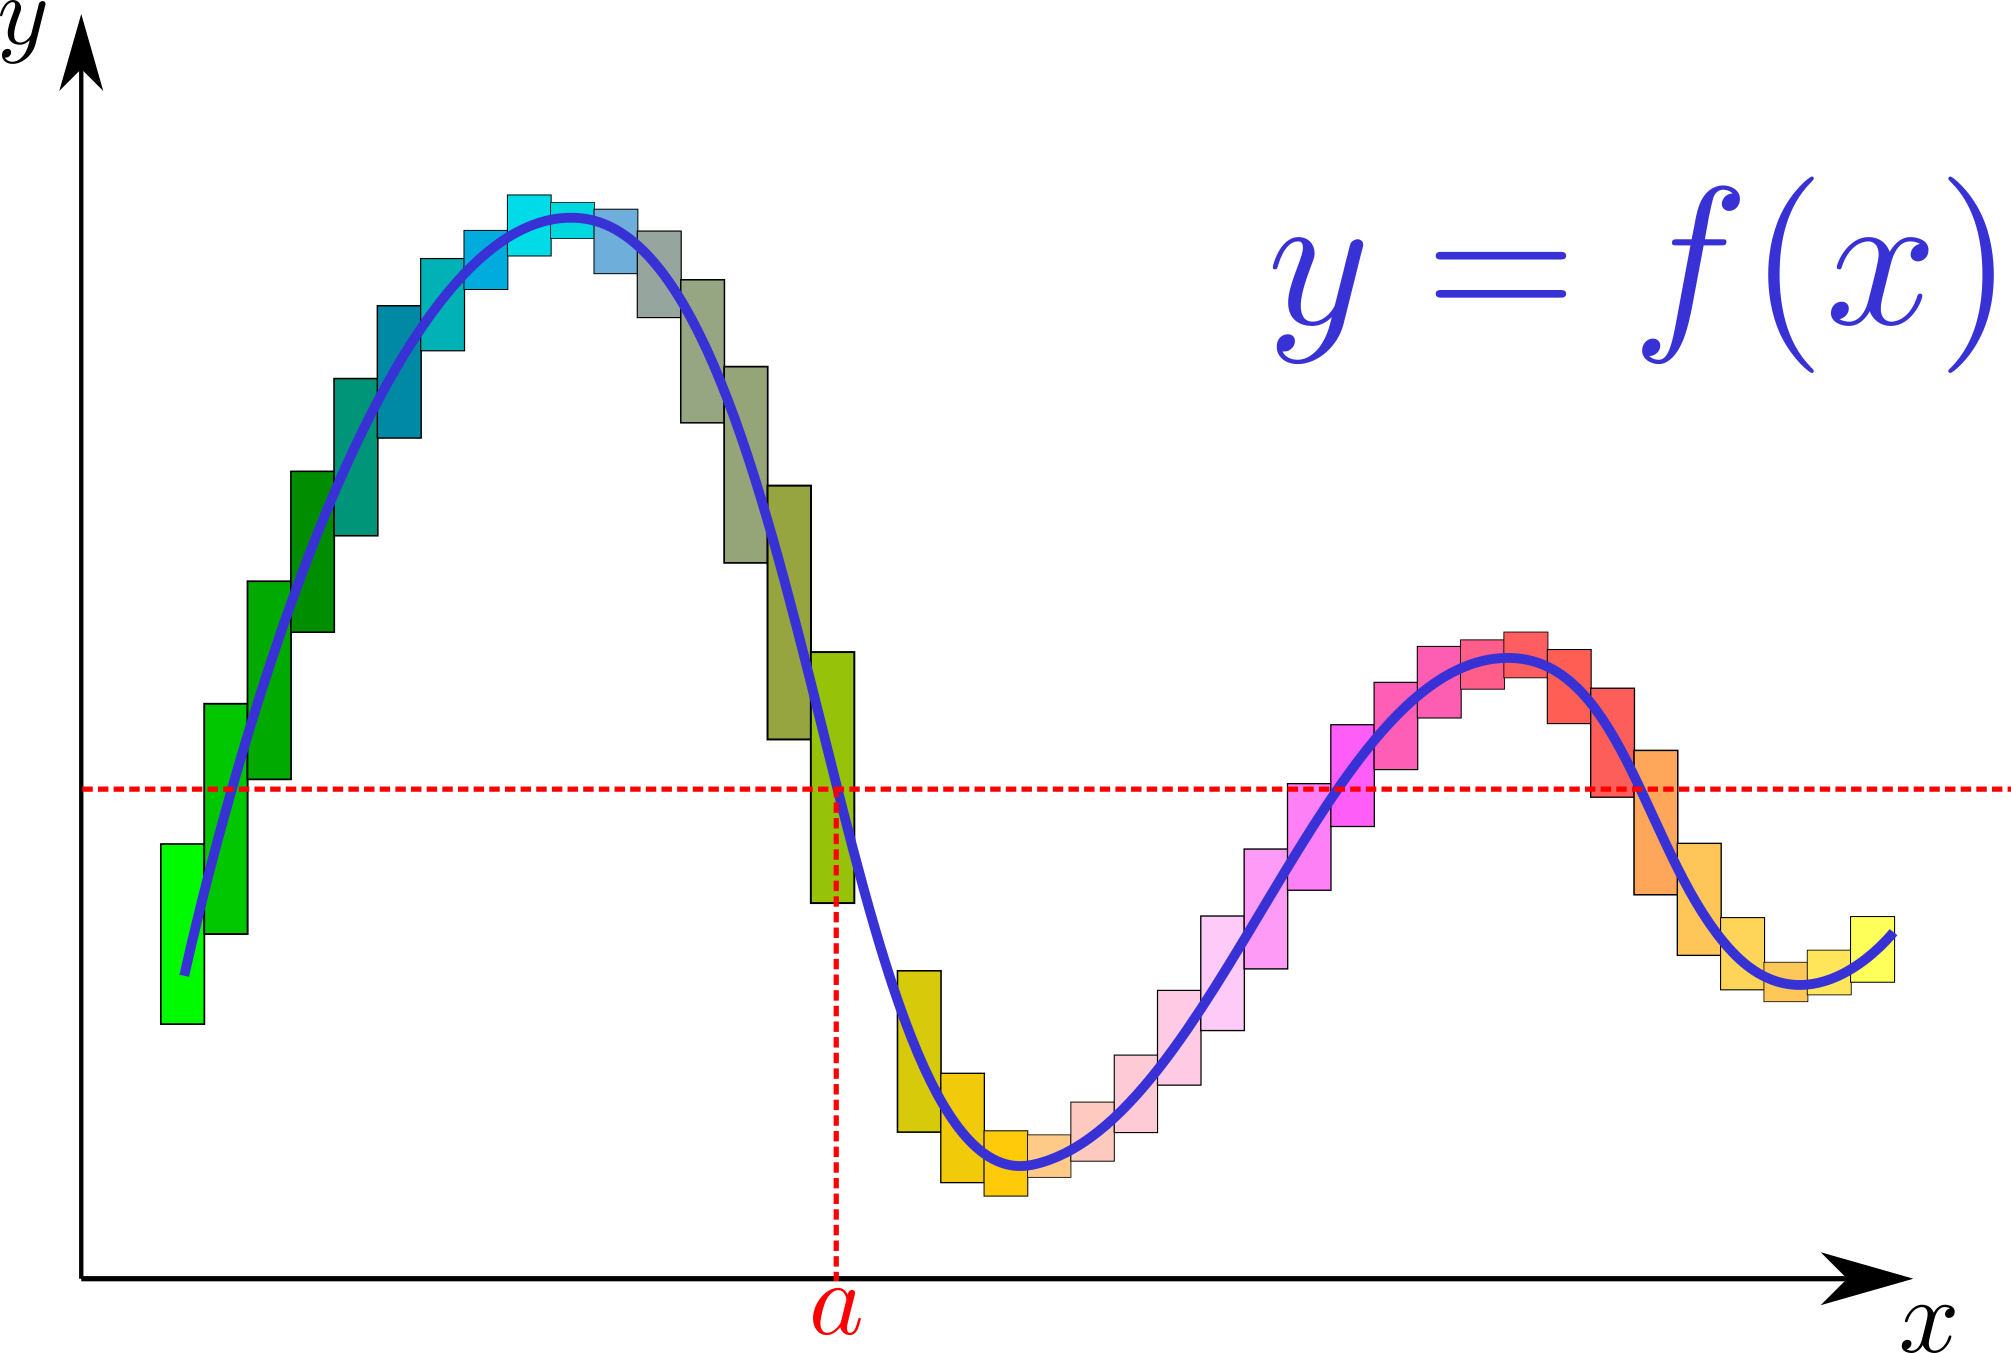
\includegraphics[scale=0.5]{images/function_optim_3.png}
            \caption{$y = f(x)$}
            \label{fig:optim3}
        \end{figure}
    }

    \only<4>{
        \begin{figure}[H]
            \centering
            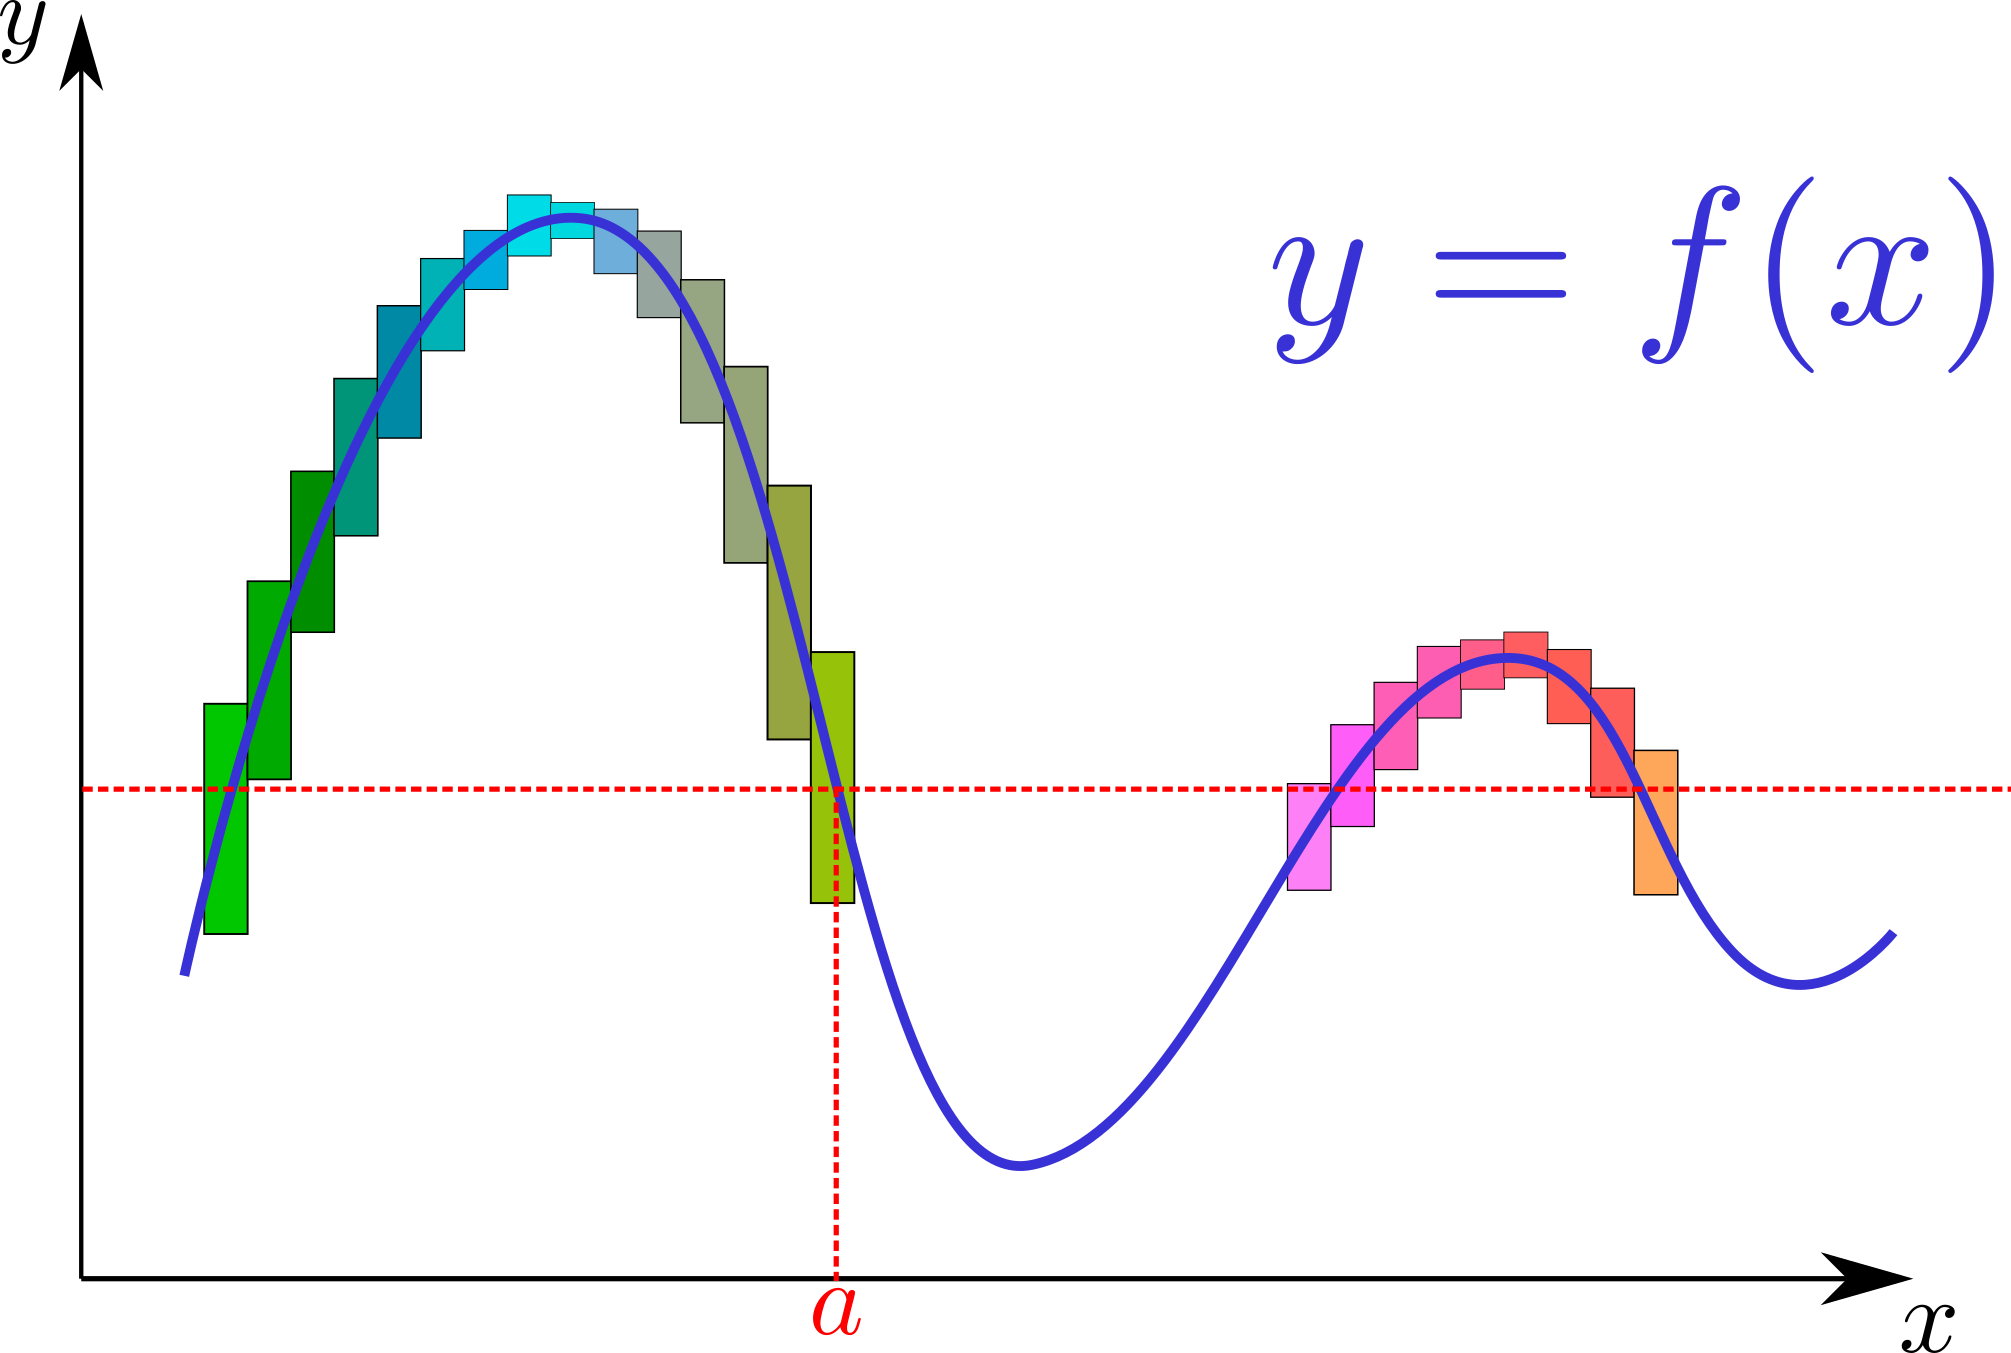
\includegraphics[scale=0.5]{images/function_optim_4.png}
            \caption{$y = f(x)$}
            \label{fig:optim4}
        \end{figure}
    }

    \only<5>{
        \begin{figure}[H]
            \centering
            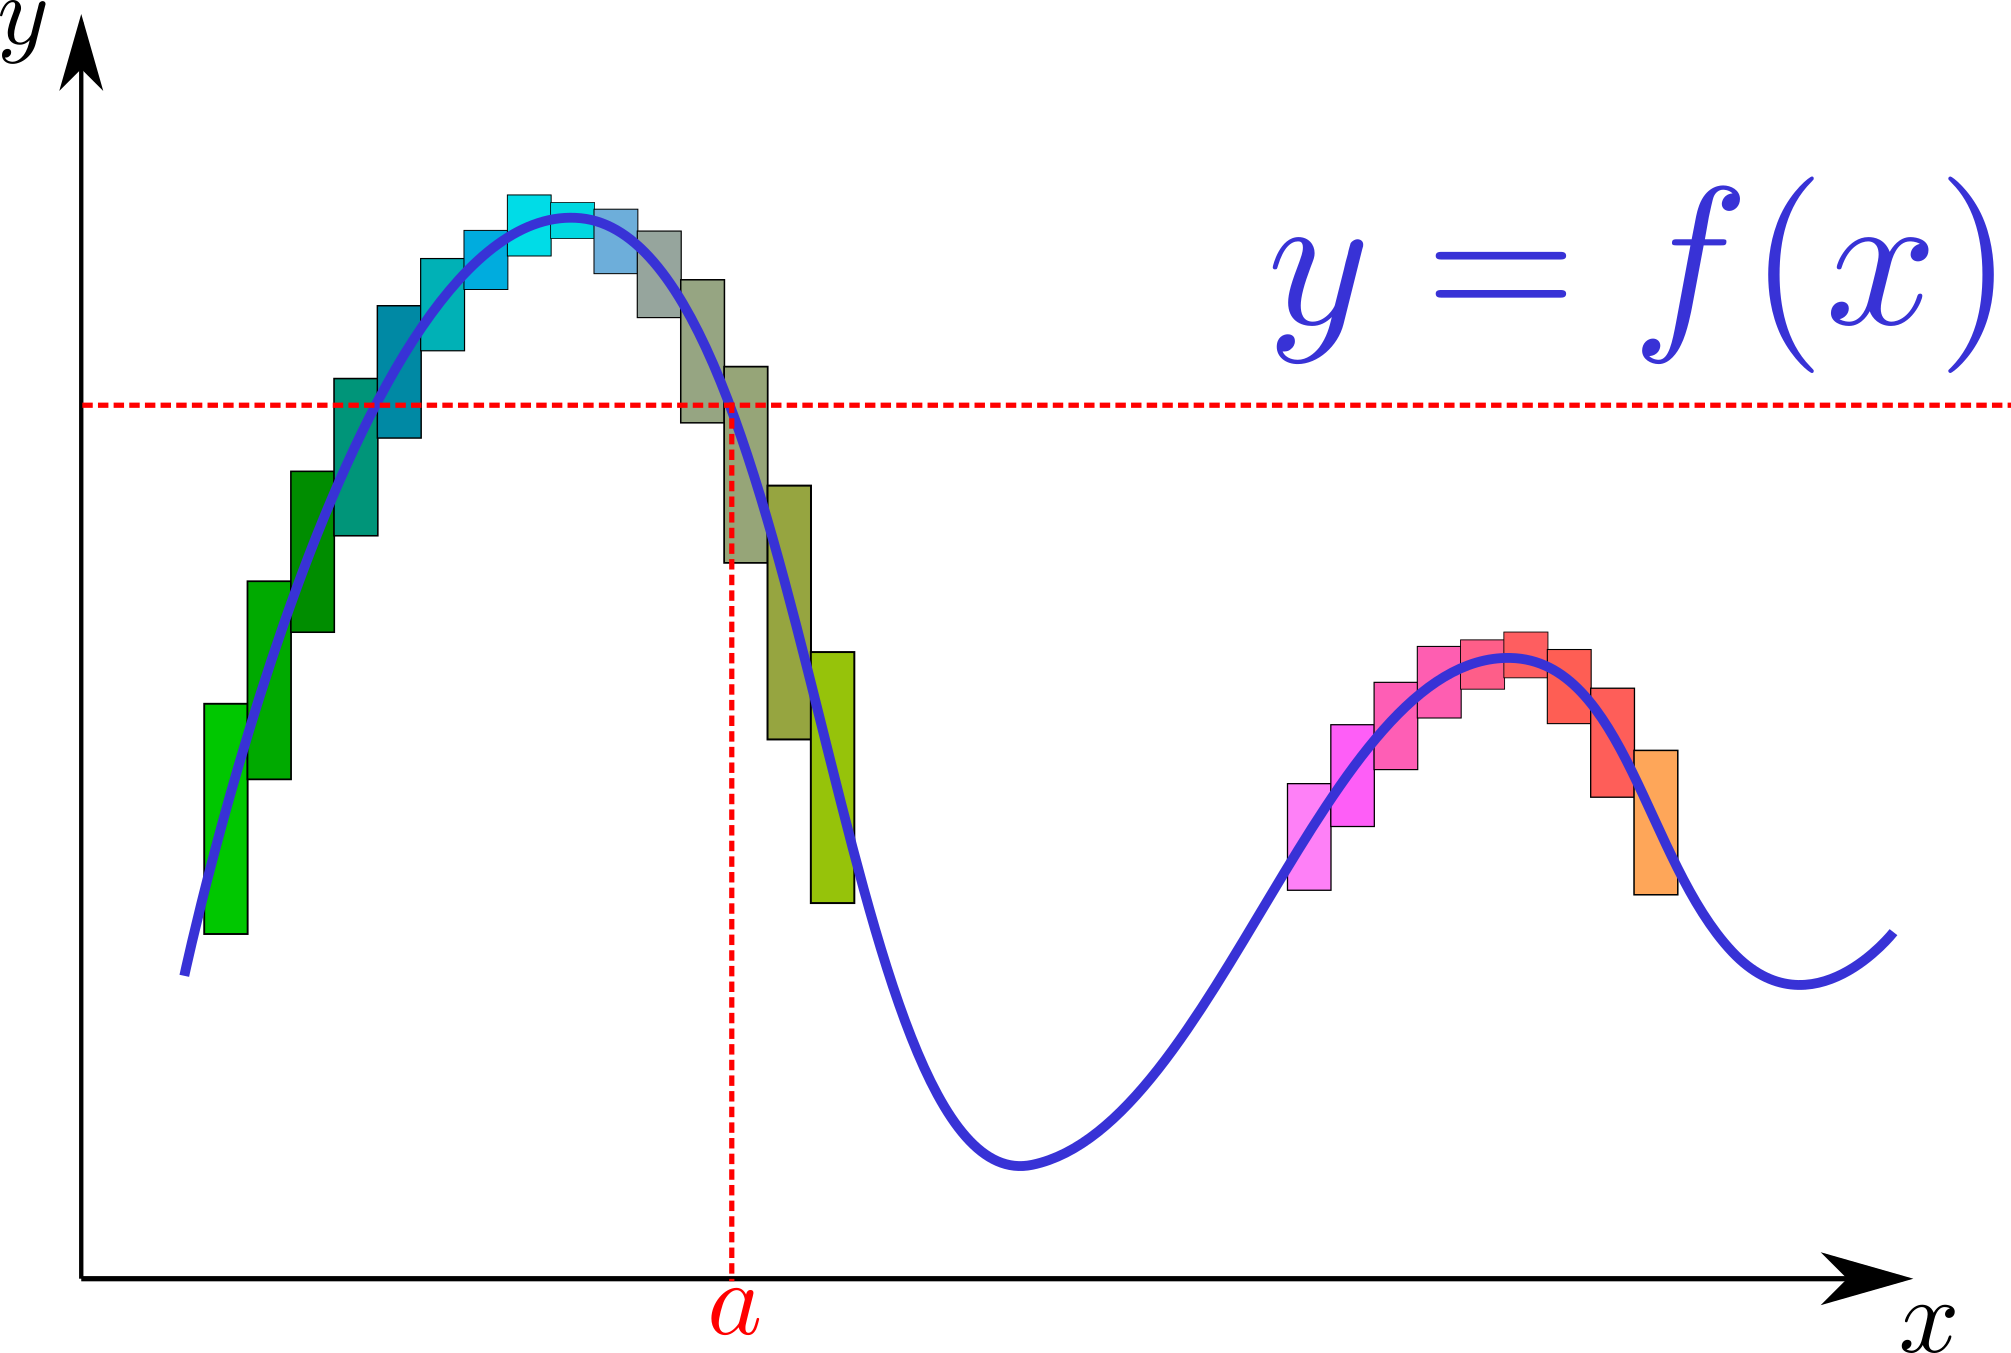
\includegraphics[scale=0.5]{images/function_optim_5.png}
            \caption{$y = f(x)$}
            \label{fig:optim5}
        \end{figure}
    }

    \only<6>{
        \begin{figure}[H]
            \centering
            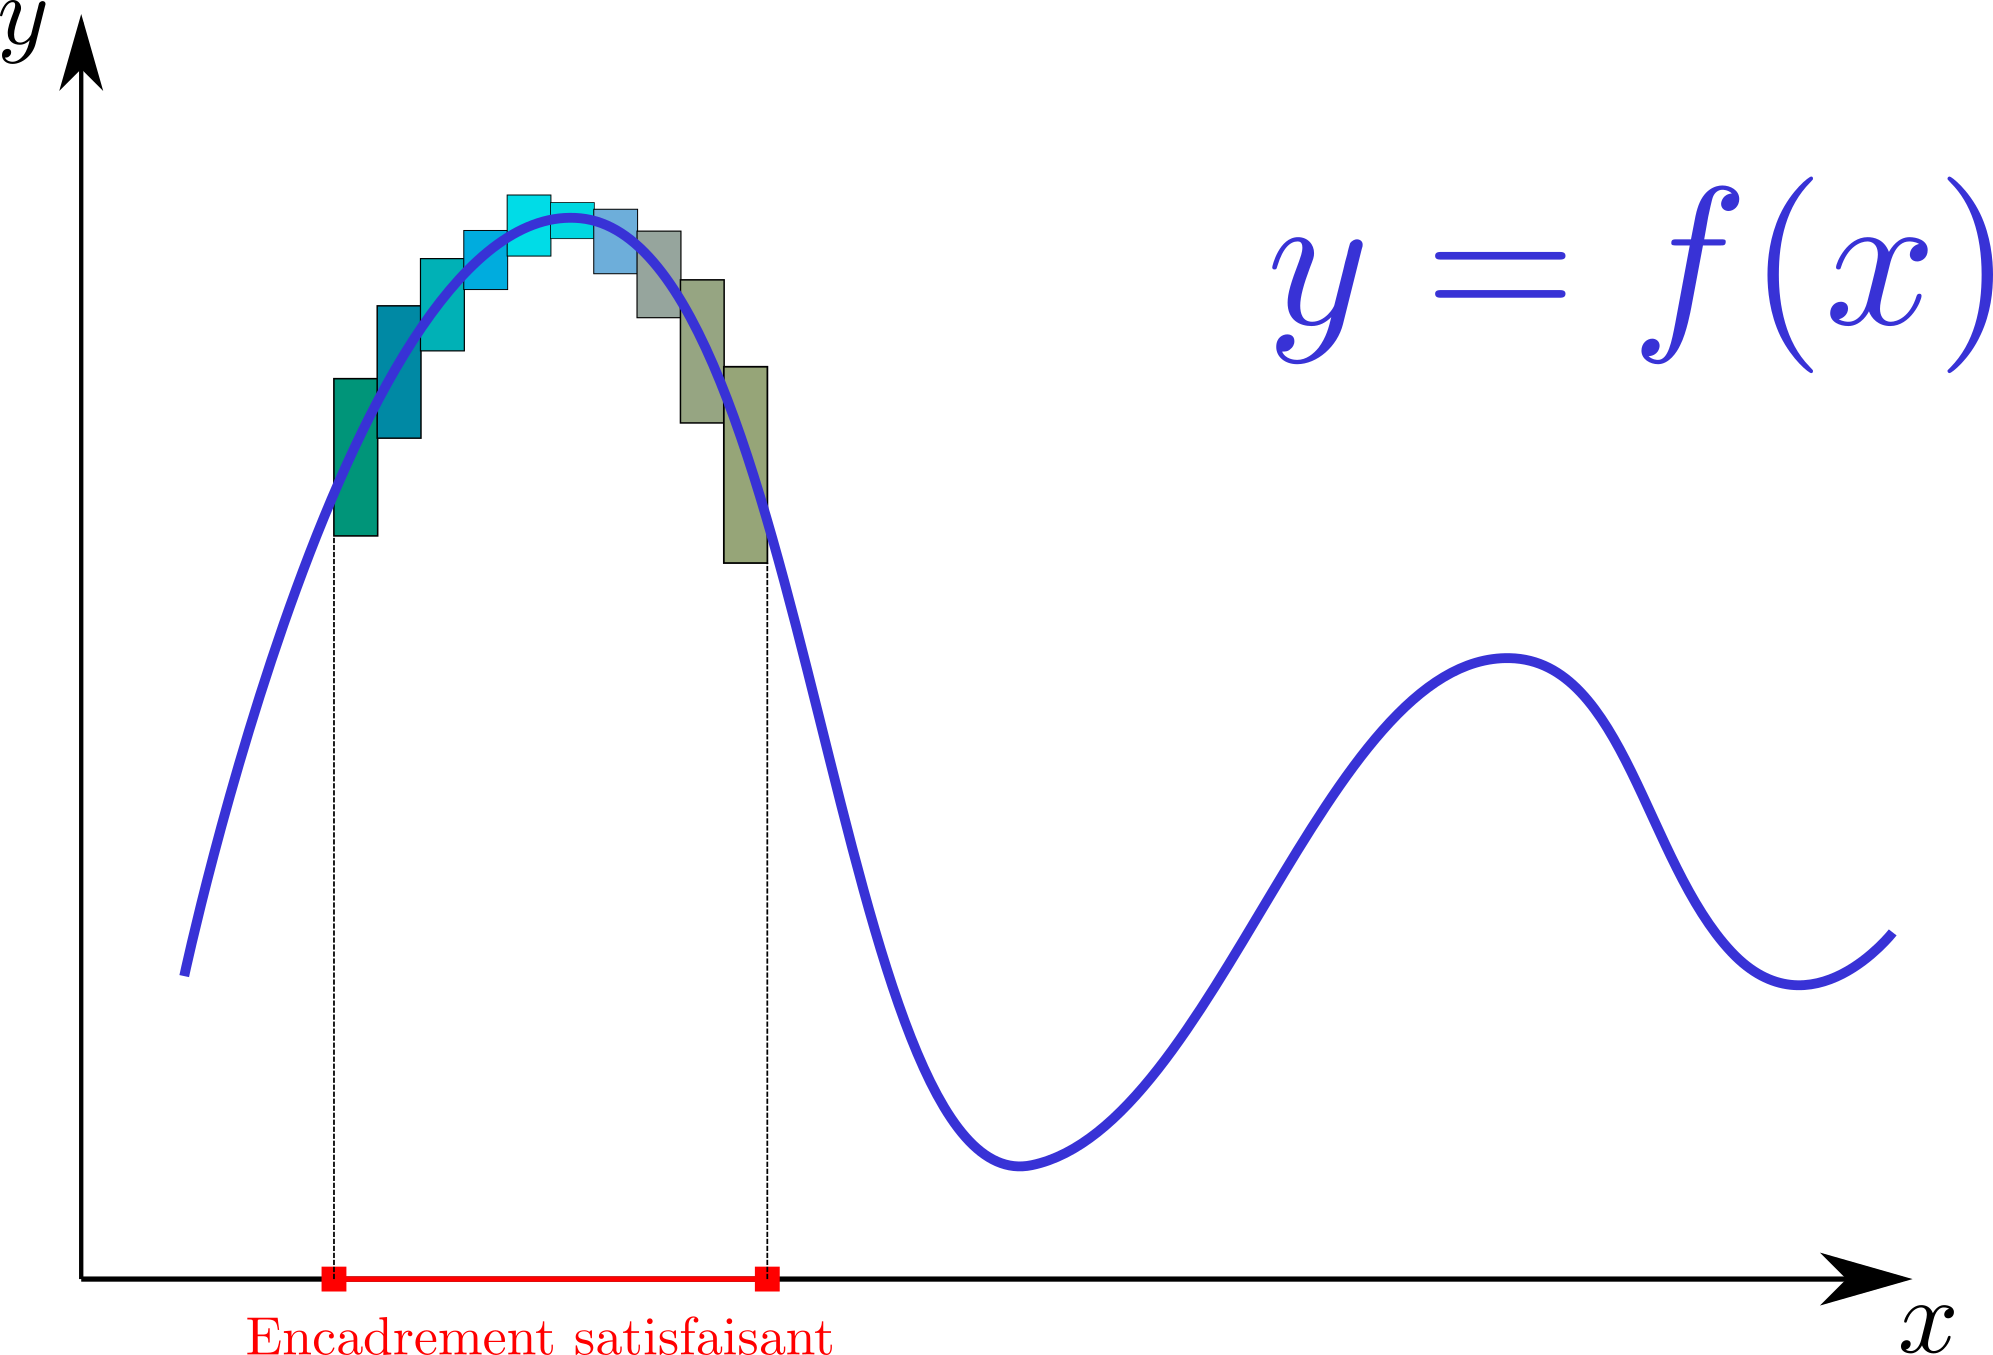
\includegraphics[scale=0.5]{images/function_optim_7.png}
            \caption{$y = f(x)$}
            \label{fig:optim7}
        \end{figure}
    }

\end{frame}



\section[3. Application à la mesure optimale]{Application à la mesure optimale}

\subsection{Optimiseur générique}
\begin{frame}
    \frametitle{3.1: Optimiseur générique}
    \begin{block}{}
        \begin{align}
            \max\limits_{\Pi = \{\Pi_j\}} I(\rho, \Pi) \\
            \Pi_j \succeq 0, \quad 1 \leq j \leq m  \\
            \displaystyle \sum_{j=1}^{m} \Pi_j = I 
        \end{align}
    \end{block}
    \begin{block}{Faisabilité}
        \begin{itemize}
            \item Fonction d'inclusion spécifique pour $x \mapsto x\log(x)$
            \item Critère de Sylvester pour la semi-définie positivité
        \end{itemize}
    \end{block}
    \pause
    \begin{block}{Temps de calcul}
        \begin{itemize}
            \item Utilisation du gradient de $I(\rho, \Pi)$: forme centrée et convexité
            \item Parallélisation de l'algorithme: gain de performance
        \end{itemize}
    \end{block}
\end{frame}


\subsection{Exemple}
\begin{frame}
    \frametitle{3.2: Exemple}
    \scriptsize
    \begin{block}{Entrées du problème}
        Deux états purs $\ket{\psi_1} = \begin{pmatrix}\frac{1}{3} \\ \frac{2 \sqrt{2}}{3}\end{pmatrix}$ et $\ket{\psi_2} = \ket{+}$, avec $p_1 = 0.1$ et $p_2 = 0.9$. Opérateurs densité correspondant:

        \begin{align}
            \rho_1 = \begin{pmatrix}
                \frac{1}{9} & \frac{2 \sqrt{2}}{9} \\ \frac{2 \sqrt{2}}{9} & \frac{8}{9}
            \end{pmatrix}, 
            \quad \rho_2 = \begin{pmatrix}
                0.5 & 0.5 \\ 0.5 & 0.5
            \end{pmatrix} \nonumber
        \end{align}

    \end{block}
    \begin{block}{Deux opérateurs de mesure inconnus}
        \begin{align}
            \Pi_1 = \begin{pmatrix}
                a_1 & b_1 + ic_1 \\ b_1 - ic_1 & d_1
            \end{pmatrix}, \quad \Pi_2 = \begin{pmatrix}
                a_2 & b_2 + ic_2 \\ b_2 - ic_2 & d_2
            \end{pmatrix} \nonumber
        \end{align}

        Information mutuelle maximum: $-0.1\log_2(0.1) - 0.9\log_2(0.9) = 0.47 \text{ Shannon}.$ 

    \end{block}
\end{frame}

\begin{frame}
    \frametitle{3.2: Exemple}
    \small
    \begin{block}{}
        On veut résoudre le problème 
        \begin{align}
            &\max\limits_{\Pi_1, \Pi_2} I(\rho_1, \rho_2, \Pi_1, \Pi_2)
        \end{align}

        tel que :

        \begin{align}
            \Pi_1 \succeq 0, \Pi_2 \succeq 0\\
            \Pi_1 + \Pi_2 = I 
        \end{align}

    \end{block}
\end{frame}

\begin{frame}
    \frametitle{3.2: Exemple}
    \small
    \begin{block}{}


        On sait que $\Pi_1 + \Pi_2 = I$, on réduit à 4 variables inconnues:

        \begin{align}
            \Pi_2 = \begin{pmatrix}
                (1-a_1) & (-b_1) + i(-c_1) \\ (-b_1) - i(-c_1) & (1-d_1)
            \end{pmatrix} \nonumber
        \end{align}

        $\rho_j$ non complexes: on enlève $c_1$.

        \medbreak

        Semi-définie positivité des $\Pi_k$ : critère de Sylvester.

        \begin{align}
            \begin{cases}
                \Pi_1 \succeq 0\\
                \Pi_2 \succeq 0
            \end{cases}
            \Leftrightarrow
            \begin{cases}
                a_1 \geq 0 \nonumber \\
                d_1 \geq 0 \nonumber \\
                a_1 \times d_1 - b_1^2 \geq 0 \nonumber \\
                (1-a_1) \times (1-d_1) - (-b_1)^2 \geq 0 \nonumber
            \end{cases}
        \end{align}
    \end{block}
\end{frame}

% Résultats (ibex / le notre)

\subsection{Résultats}
\begin{frame}
    \frametitle{3.3: Résultats}
% \scriptsize
    \begin{block}{Ibex}
\begin{itemize}
    \item Information mutuelle optimale : $0.0681 \text{ Shannon}$
    \item Temps de calcul : 87 secondes, précision relative: $10^{-3}$.
    \item Solutions optimales: \\ $\Pi_1 = \begin{pmatrix} 0.454 & -0.498 \\ -0.498 & 0.546 \end{pmatrix}$, \quad $\Pi_2 = \begin{pmatrix}0.546 & 0.498 \\ 0.498 & 0.454 \end{pmatrix}$.
\end{itemize}
    \end{block}

    \begin{block}{Notre solveur}

        \begin{itemize}
            \item Information mutuelle optimale : $0.0681 \text{ Shannon}$
            \item Temps de calcul : 13 secondes, précision relative: $10^{-8}$.
            \item Solutions optimales: \\ $\Pi_1 = \begin{pmatrix} 0.454 & -0.498 \\ -0.498 & 0.546 \end{pmatrix}$, \quad $\Pi_2 = \begin{pmatrix}0.546 & 0.498 \\ 0.498 & 0.454 \end{pmatrix}$.
        \end{itemize}

    \end{block}

\end{frame}


\section[Conclusion]{Conclusion}
\begin{frame}
    \frametitle{Conclusion}

    Contribution:

    Réalisation d'un solveur générique pour le problème de la détection optimale quantique, via le calcul par intervalle, avec pour critère l'information mutuelle.

    \medbreak
    
    Perspectives:
    \begin{enumerate}

        \item Utilisations d'autres formes de fonction d'inclusion pour contrer des temps de calcul qui deviennent grands: forme centrée, arithmétique des pentes.
        \item \'Etendre le problème en ajoutant du bruit sur le canal de communication;

    \end{enumerate}
\end{frame}

\begin{frame}
    \begin{center}
        Merci pour votre attention !
    \end{center}

    \begin{figure}
        \centering
        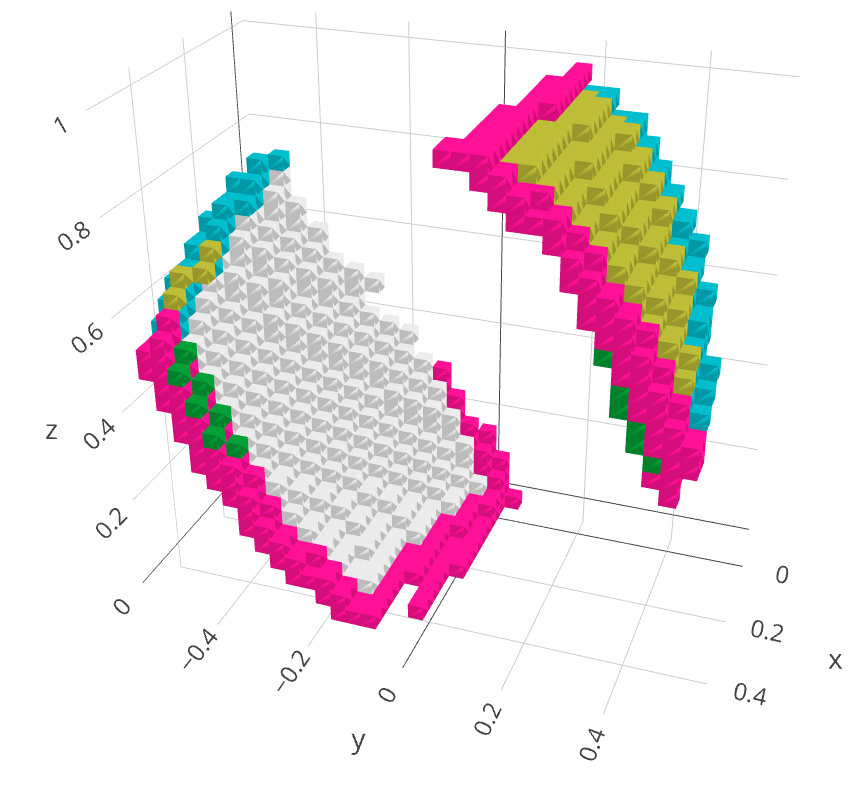
\includegraphics[scale=0.2]{images/illustration_boites.png}
    \end{figure}
\end{frame}


\end{document}